%%
%% This is file `example.tex',
%% generated with the docstrip utility.
%%
%% The original source files were:
%%
%% coppe.dtx  (with options: `example')
%% 
%% This is a sample monograph which illustrates the use of `coppe' document
%% class and `coppe-unsrt' BibTeX style.
%% 
%% \CheckSum{1613}
%% \CharacterTable
%%  {Upper-case    \A\B\C\D\E\F\G\H\I\J\K\L\M\N\O\P\Q\R\S\T\U\V\W\X\Y\Z
%%   Lower-case    \a\b\c\d\e\f\g\h\i\j\k\l\m\n\o\p\q\r\s\t\u\v\w\x\y\z
%%   Digits        \0\1\2\3\4\5\6\7\8\9
%%   Exclamation   \!     Double quote  \"     Hash (number) \#
%%   Dollar        \$     Percent       \%     Ampersand     \&
%%   Acute accent  \'     Left paren    \(     Right paren   \)
%%   Asterisk      \*     Plus          \+     Comma         \,
%%   Minus         \-     Point         \.     Solidus       \/
%%   Colon         \:     Semicolon     \;     Less than     \<
%%   Equals        \=     Greater than  \>     Question mark \?
%%   Commercial at \@     Left bracket  \[     Backslash     \\
%%   Right bracket \]     Circumflex    \^     Underscore    \_
%%   Grave accent  \`     Left brace    \{     Vertical bar  \|
%%   Right brace   \}     Tilde         \~}
%%
\documentclass[dsc]{coppe}
\usepackage{amsmath,amssymb}
\usepackage{hyperref}

\makelosymbols
\makeloabbreviations

\begin{document}
  \title{Motivando Mulheres em Cursos STEM por meio de Narrativa: a jornada de aprendizagem da heroína}
  \foreigntitle{Thesis Title}
  \author{Luis Felipe}{Coimbra Costa}
  \advisor{Prof.}{Geraldo}{Xexéo}{D.Sc.}
  \advisor{Prof.}{Ana Moura}{Santos}{Ph.D.}
  

  \examiner{Prof.}{Nome do Primeiro Examinador Sobrenome}{D.Sc.}
  \examiner{Prof.}{Nome do Segundo Examinador Sobrenome}{Ph.D.}
  \examiner{Prof.}{Nome do Terceiro Examinador Sobrenome}{D.Sc.}
  \examiner{Prof.}{Nome do Quarto Examinador Sobrenome}{Ph.D.}
  \examiner{Prof.}{Nome do Quinto Examinador Sobrenome}{Ph.D.}
  \department{PEC}
  \date{02}{2011}

  \keyword{Primeira palavra-chave}
  \keyword{Segunda palavra-chave}
  \keyword{Terceira palavra-chave}

  \maketitle
  \frontmatter
  \dedication{A algu\'em cujo valor \'e digno desta dedicat\'oria.}

  \chapter*{Agradecimentos}

  Gostaria de agradecer a todos.

  \begin{abstract}

  Apresenta-se, nesta tese, ...

  \end{abstract}

  \begin{foreignabstract}

  In this work, we present ...

  \end{foreignabstract}

  \tableofcontents
  \listoffigures
  \listoftables
  \printlosymbols
  \printloabbreviations

  \mainmatter
\chapter{Introdução}

Essa tese, cuja finalidade é incentivar a presença de mulheres em cursos Ciências, Tecnologias, Engenharias e Matemática, conhecidas também pelo acrônimo inglês de "STEM", está sendo apresentado por um homem. Isso pode gerar alguns questionamentos quanto ao meu lugar de fala no processo. Durante todo o trabalho, mulheres foram ouvidas, e também participaram da construção das bases teóricas, do desenvolvimento do framework e de todo o processo de desenvolvimento da proposta. Considero que este processo coletivo de ideias seja também importante para engajar os homens nessa busca do equilíbrio e diálogo entre as decisões de pesquisa relacionadas ao campo da igualdade de gênero, para que os resultados de tais decisões sejam também mais equilibrados e assertivas. Não é somente aumentando o número de mulheres nas áreas de STEM que vamos conseguir resolver a questão da igualdade de gênero, mas também permitindo com que toda a concepção, análise e resultados das pesquisas, nestas áreas, sejam amplos o suficientes para que o diálogo e as ideais sejam também melhor explorados pelas diversas visões e pontos de vistas de homens e mulheres, principalmente levando-se em consideração que as experiências vividas, o ambiente cultural e os contextos políticos e educacionais são bem diferentes entre homens e mulheres.

Este capítulo apresenta o estudo e está organizado nas seguintes seções: Contexto de pesquisa, Declaração do problema, Objetivos de pesquisa, Contribuições de pesquisa, Publicações e Metodologia de pesquisa.

\section{Contexto de Pesquisa}

As tecnologias de informação, aliadas ao desenvolvimento da Internet, transformaram definitivamente o modo em que vivemos \citep{valente_tecnologia_2018}. Apesar disso, ainda existe um processo de mudança na área da educação que apresenta muitas resistências. 

Nos dias atuais, os alunos possuem uma maior facilidade de acessar conteúdos didáticos, em função da Internet e suas aplicações, como tutorias online ou \textit{streaming} de vídeo. Esta forma de obter informações pode ajudar o discente a desenvolver seu processo de aprendizagem de maneira mais autônoma.

A questão, portanto, não é alterar os conteúdos disciplinares, mas, sim, a maneira como eles devem ser trabalhados \citep{valente_tecnologia_2018}.

\section{Declaração do Problema}

\section{Objetivos de Pesquisa}


\section{Contribuições de pesquisa}


\section{Publicações}

\subsection{Trabalhos publicados em anais de eventos (completo)}


\begin {itemize}
    \item\textbf {Bernardo Tauce; COSTA, L. F. C.
Uma análise crítica sobre canvas para jogos, baseado nas qualidades do Business Model Canvas e
Design Thinking Canvas. XI SIMPÓSIO BRASILEIRO DE JOGOS E ENTRETENIMENTO DIGITAL. , v.XVII, p.www.sbgames.org - , 2018.}
     \item\textbf {COSTA, L. F. C.; SOBRAL, A.; ANDRADE, H.
Software Público Regional: Conectando o Mecanismo Colaborativo Regional entre países da América
Latina e Caribe. Simpósio de História da Informática na América Latina e Caribe. , v.V, p.www.shialc.org - ,2018.}
     \item\textbf {XEXÉO, GERALDO; MANGELI, EDUARDO; SILVA, FARMY; OURIQUES, LEANDRO; COSTA,LUIS FELIPE COIMBRA; MONCLAR, RAFAEL STUDART
Games as Information Systems In: SBSI 2021: XVII Brazilian Symposium on Information Systems, 2021,
Uberlândia Brazil. XVII Brazilian Symposium on Information Systems. , 2021. p.1 -}
     \item\textbf {SANTOS, ANA MOURA; SA, SOFIA; COSTA, LUIS FELIPE C.; COHEUR, LUISA
Setting up Educational Escape Games: Lessons learned in a Higher Education setting In: 2021 4th
International Conference of the Portuguese Society for Engineering Education (CISPEE), 2021, Lisbon.
2021 4th International Conference of the Portuguese Society for Engineering Education (CISPEE).
IEEE, 2021. p.1 -}
     \item\textbf {COSTA, L.; SANTOS; 2020. Linear Algebra Flipped Classroom with a MOOC. 4th
International Conference of the Portuguese Society for Engineering Education (CISPEE 2020).
IEEE, 2021. p.1 -}
    \item\textbf {ROCHA, JOSE BERNARDO; COSTA, LUIS FELIPE COIMBRA; PRADA, RUI; SILVA, ANTONIO
RITO; GONCALVES, DANIEL; CORREIA, PEDRO
Quizzes (As a Tool for Self-Regulated Learning) in Software Engineering Education In: 2020 IEEE 32nd
Conference on Software Engineering Education and Training (CSEET), 2020, Virtual Conference.
2020 IEEE 32nd Conference on Software Engineering Education and Training (CSEET). IEEE,
2020. p.1 -}
    \item\textbf {PINTO, MARCOS RODRIGUES; BARBOSA, CARLOS EDUARDO; DE LIMA, YURI OLIVEIRA;
COIMBRA COSTA, LUIS FELIPE; DE SOUZA, JANO MOREIRA
A Service Bus for Knowledge Management Systems in Brazilian Federal Government In: 2019 IEEE 23rd
International Conference on Computer Supported Cooperative Work in Design (CSCWD), 2019, Porto.
2019 IEEE 23rd International Conference on Computer Supported Cooperative Work in Design
(CSCWD). , 2019. p.111 -}
    \item\textbf {CASTRO, DIEGO CARDOSO BORDA; BARBOSA, CARLOS EDUARDO; COSTA, LUIS FELIPE
COIMBRA; SOUZA, JANO
Analyzing the impact of Technological KM and Participatory KM in FTA (S) In: The 31st International Conference on Software Engineering and Knowledge Engineering, 2019, Lisboa, 2019. p.770 -}
\end {itemize}


\subsection{Trabalhos publicados em anais de eventos (resumo)}


\begin {itemize}
    \item\textbf {COSTA, L. F. C.; SANTOS, A. M.; DE LIMA, YURI OLIVEIRA; XEXÉO, GERALDO
Creating new narratives for women in STEM: Heroine's Learning Journey In: 20th Gender Summit - LAC,
2021}
    \item\textbf {Creating new narratives for women in STEM: Heroine's Learning Journey. , 2021.
DE LIMA, YURI OLIVEIRA; COSTA, L. F. C.; SANTOS, A. M.; DE SOUZA, JANO MOREIRA}
     \item\textbf {COSTA, L. F. C.; SANTOS, A. M.; XEXÉO, GERALDO
The Heroine's Learning Journey applied to a MOOC: Machine Learning, Maths and Ethics. In: 2021 4th
International Conference of the Portuguese Society for Engineering Education (CISPEE), 2021, Lisbon.
2021 4th International Conference of the Portuguese Society for Engineering Education (CISPEE).
, 2021.}
\end {itemize}


\subsection{Trabalhos técnicos}

\begin {itemize}
    \item\textbf {XEXEO, G.; COSTA, L. F. C.
O Que São Jogos - Uma Introdução ao Objeto de Estudo do Ludes, 2017}
    \item\textbf {BARBOSA, C. E.; LIMA, Y.; COSTA, L. F. C.; LUIS FELIPE COSTA
Working in 2050: A view of how changes on the work will affect the society. Laboratório do Futuro,}
\end {itemize}

\subsection{Demais produções técnicas}


\begin {itemize}
    \item\textbf {SANTOS, A. M.; COSTA, L. F. C.
LearningAnaytics-MOOC Técnico 2020, 2020. (Relatório de pesquisa)}
\end {itemize}



\section{Metodologia de Pesquisa}

\begin{figure}
    \centering
    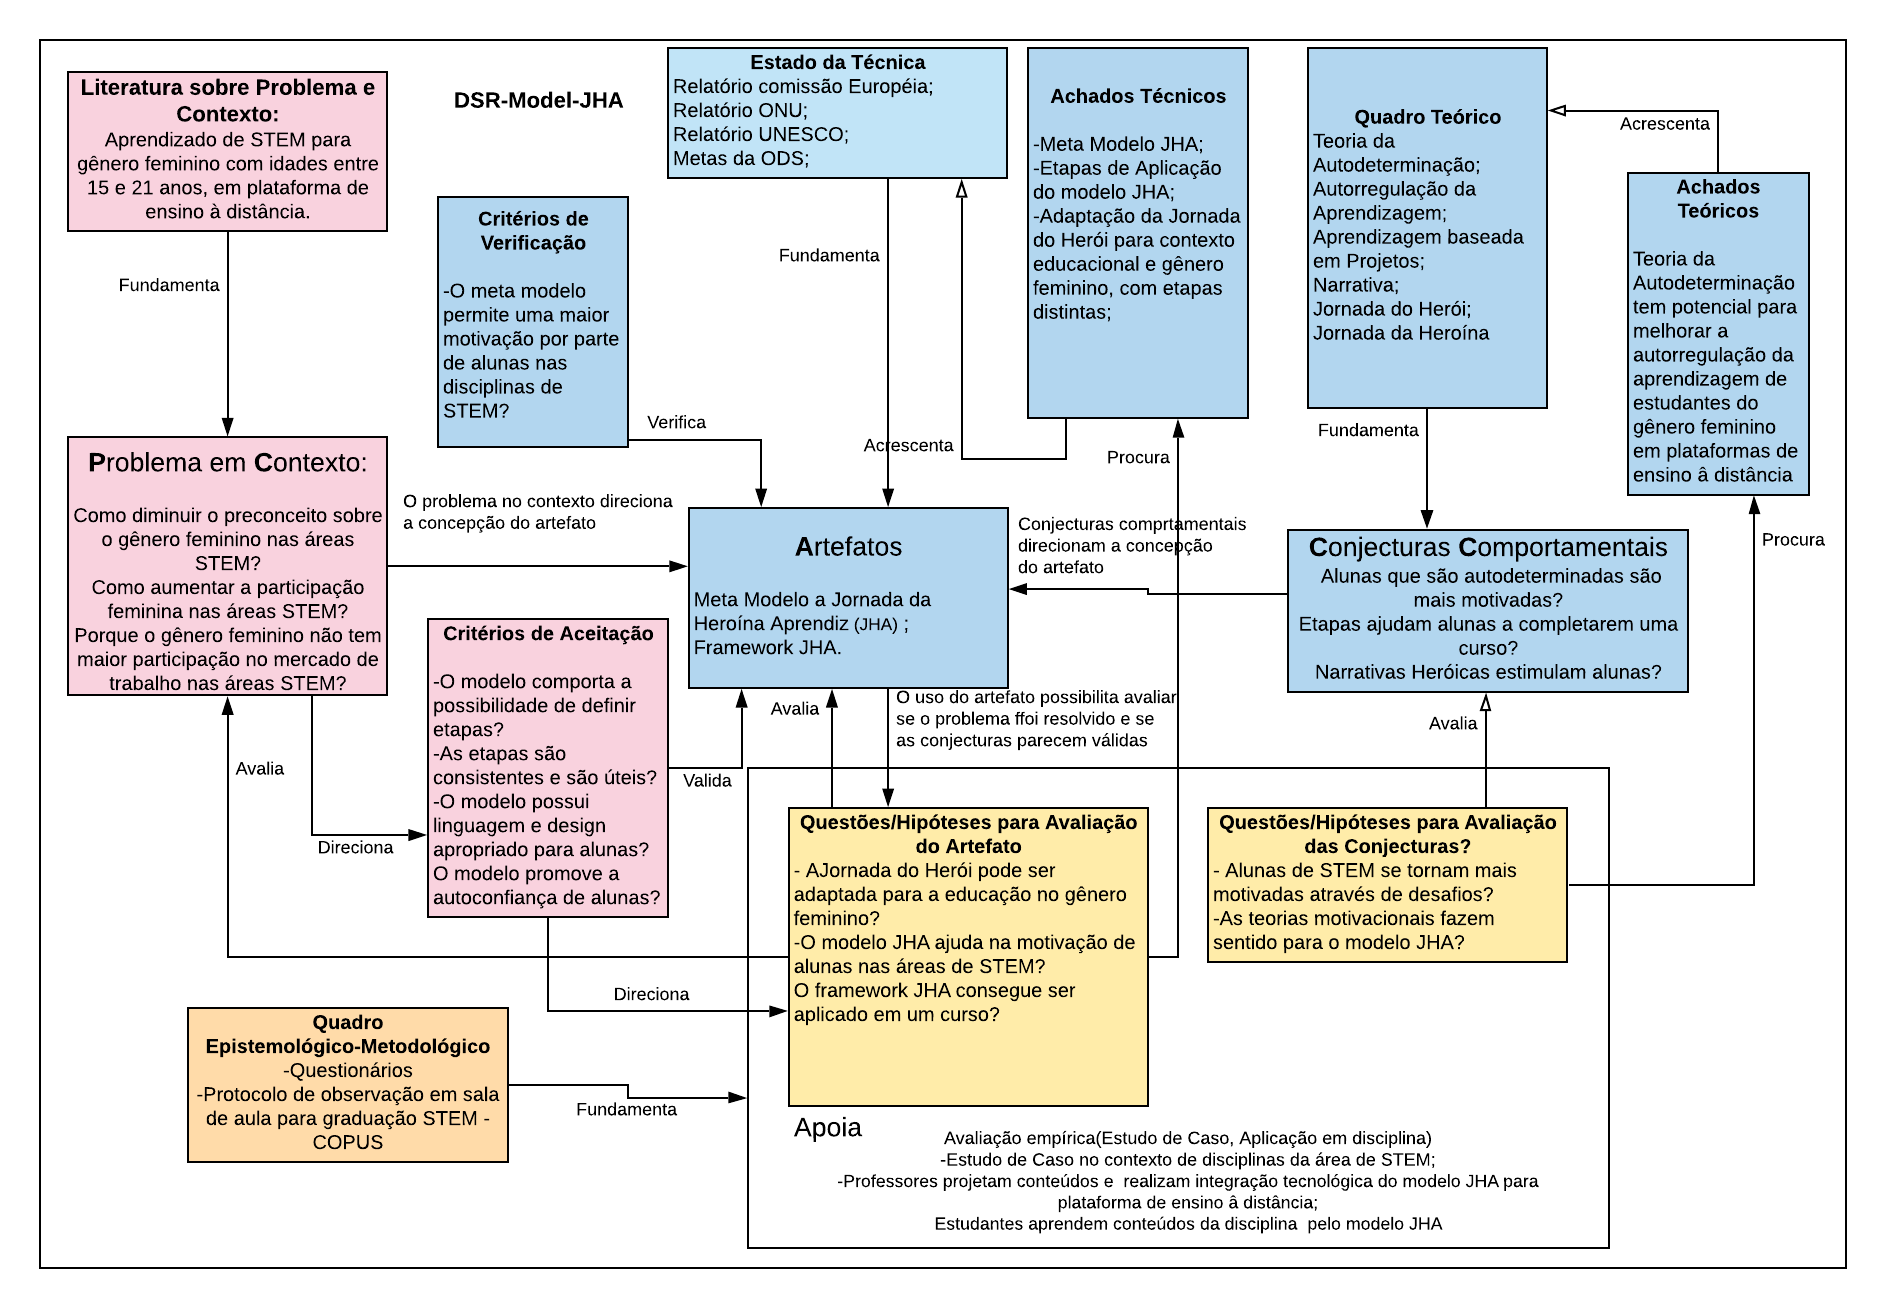
\includegraphics[width=.9\textwidth]{chaps/Images/DSRV2.png}
    \caption{Design Science Research}
    \label{fig:dsr}
\end{figure}

Uma das questões de pesquisa que importa para este estudo é: Como motivar estudantes do gênero feminino a aprenderem a se orientar por uma aprendizagem investigativa e autorregulada, utilizando recursos tecnológicos e superando desafios de forma planejada?

Literatura sobre Problema e Contexto:
Aprendizado de STEM para gênero feminino com idades entre 15 e 21 anos, em plataforma de ensino à distância.

Problema em Contexto:

Como diminuir o preconceito sobre o gênero feminino nas áreas STEM?
Como aumentar a participação feminina nas áreas STEM?
Porque o gênero feminino não tem maior participação no mercado de trabalho nas áreas STEM?

Critérios de Aceitação

-O modelo comporta a possibilidade de definir etapas?
-As etapas são consistentes e são úteis?
-O modelo possui linguagem e design apropriado para alunas? 
O modelo promove a autoconfiança de alunas?

Critérios de Verificação

-O meta modelo permite uma maior motivação por parte de alunas nas disciplinas de STEM?

Estado da Técnica
Relatório comissão Européia;
Relatório ONU;
Relatório UNESCO; 
Metas da ODS;

Achados Técnicos

-Meta Modelo JHA;
-Etapas de Aplicação do modelo JHA;
-Adaptação da Jornada do Herói para contexto educacional e gênero feminino, com etapas distintas;


Quadro Teórico
Teoria da Autodeterminação;
Autorregulação da Aprendizagem;
Aprendizagem baseada em Projetos;
Narrativa;
Jornada do Herói;
Jornada da Heroína

Achados Teóricos

Teoria da Autodeterminação tem potencial para melhorar a autorregulação da aprendizagem de estudantes do gênero feminino em plataformas de ensino â distância

Conjecturas Comportamentais
 Alunas que são autodeterminadas são mais motivadas?
Etapas ajudam alunas a completarem uma curso?
Narrativas Heróicas estimulam alunas?  

Artefatos 

Meta Modelo a Jornada da Heroína Aprendiz (JHA) ;
Framework JHA.

Quadro Epistemológico-Metodológico
-Questionários
-Protocolo de observação em sala de aula para graduação STEM - COPUS

Questões/Hipóteses para Avaliação do Artefato
- AJornada do Herói pode ser adaptada para a educação no gênero feminino?
-O modelo JHA ajuda na motivação de alunas nas áreas de STEM?
O framework JHA consegue ser aplicado em um curso?


Questões/Hipóteses para Avaliação das Conjecturas?
- Alunas de STEM se tornam mais motivadas através de desafios?
-As teorias motivacionais fazem sentido para o modelo JHA?

\section{Estrutura do documento de Tese}





\chapter{Investigações preliminares em motivação em ensino STEM}

Este capítulo descreve as investigações preliminares que foram realizadas com intenção de verificar o ensino de STEM, em especial a motivação destes estudantes e a questão da igualdade de gênero nestas áreas. Na seção 2.1 é apresentado o estado atual da participação feminina nas áreas de STEM, algumas iniciativas que visam melhorar a lacuna existente e também é detalhado o projeto criado a partir da tese e em parceria entre a UFRJ e o IST, denominado igualdade STEM. Na seção 2.2, é apresentado uma revisão em torno das principais teorias motivacionais aplicadas na área da educação em estudantes de STEM, principalmente a Teoria da Autodeterminação e a Teoria de Metas. Na seção 2.3, é apresentado o resultado das pesquisas relativas a quizzes aplicados em autorregulação da aprendizagem, através de um mapeamento sistemático. Na seção 2.4, é apresentado o as principais caraterísticas de plataformas de ensino online, em especial as plataforma de MOOC. Na seção 2.5, são apresentados os principais conceitos sobre narrativas e sua aplicação nas áreas da educação. Por último, na Seção 2.6 são feitas as considerações finais do capítulo.


\section{O Projeto IgualdadeStem}

Nos últimos anos, a diferença de gênero diminuiu globalmente, mas ainda há um longo caminho a percorrer até a paridade. No ritmo atual, levará 99,5 anos para fechar a lacuna globalmente e 59 anos para fazê-lo na América Latina. No Brasil, a matrícula feminina no ensino superior aumentou, mas a participação em programas STEM ainda é baixa quando comparada com a dos homens. A lacuna na educação STEM, considerada essencial para o futuro do trabalho, é um desafio que deve ser enfrentado para que a paridade econômica de gênero algum dia seja alcançada. Este estudo tem como objetivo apresentar dados secundários sobre a igualdade de gênero em STEM no Brasil, bem como um levantamento, com base em dados primários, de iniciativas que buscam promover a igualdade de gênero na educação STEM no Brasil. A estrutura proposta pelo projeto UNESCO STEM e Avanço de Gênero foi usada para coletar dados secundários sobre igualdade de gênero e apresentar as iniciativas. Os resultados de nosso estudo podem ser usados para comparar o caso brasileiro com outros países em termos do estado atual da igualdade de gênero no Ensino Superior STEM, bem como as iniciativas para diminuir a lacuna de gênero. O documento também pode ser usado para ajudar os interessados em desenvolver iniciativas para a igualdade de gênero em STEM a entender quais problemas eles querem ajudar a resolver, comparando seus objetivos com os levantados em nosso trabalho.

\subsection{Introdução}

As áreas de Ciência, Tecnologia, Engenharia e Matemática (STEM) são consideradas fundamentais para o Futuro do Trabalho a partir de evoluções em tecnologias como Inteligência Artificial, Robótica, Internet das Coisas e tantas outras que fazem parte da 4ª Revolução Industrial. Estar preparado como sociedade para um futuro inclusivo e justo implica proporcionar oportunidades de Educação e Trabalho a todos os grupos sociais. A distância entre mulheres e homens é muito grande em termos de acesso ao ensino superior na área de STEM em países desiguais como o Brasil. A análise do hiato de gênero e a criação de iniciativas que ajudem a reduzir esse problema são essenciais para caminharmos em direção a uma sociedade mais igualitária. A diferença de gênero está sendo reduzida lentamente em todo o mundo. No ritmo atual, a igualdade de gênero só deve ser alcançada em 99,5 anos \citep{schwab_global_2019}. A situação é particularmente preocupante na área STEM. Na Europa, por exemplo, as instituições de ensino superior, como as que fazem parte do projeto Fostering Women to STEM MOOCs (FOSTWOM), preocupam-se com o problema da baixa percentagem de diplomados em STEM e a consequente diminuição do número de mulheres a exercer profissões em STEM áreas [2]. Nos países nórdicos, a porcentagem de jovens graduados STEM é de aproximadamente 20\% \citep{noauthor_2018_nodate}. Na Itália e no Reino Unido, esse percentual chega a 30\%, mas são poucas as mulheres que exercem uma profissão científico-tecnológica \citep{noauthor_2018_nodate}. Em muitos países, existe uma forte pressão para que as mulheres interessadas em ciências e matemática se dirijam às áreas da Saúde \citep{noauthor_2018_nodate}. Apesar de ocupar a 92ª posição em um ranking de igualdade de gênero \citep{schwab_global_2019}, o Brasil fornece evidências de que ainda precisa dar o primeiro passo para aceitar que o problema existe e precisa ser enfrentado, visto que 12\% das pessoas são contra o aumento de gênero igualdade no país enquanto 21\% consideram que nenhuma mudança é necessária [4]. Os desafios da igualdade de gênero no país encontram-se principalmente nos setores de empoderamento político, visto que a participação das mulheres no parlamento é de apenas 15\%, e nas oportunidades econômicas, onde o número de mulheres no mercado de trabalho tem crescido, mas a a desigualdade salarial ainda é grande \citep{schwab_global_2019}. Um número que exemplifica o tamanho do desafio corporativo no Brasil é que apenas 0,8\% das empresas têm mulheres CEOs e apenas 8,6\% dos assentos nos conselhos de administração são ocupados por mulheres [4].

Considerando a formação em STEM, os dados de universitários no Brasil mostram uma baixa participação de apenas 30\% das mulheres nos cursos de STEM. Observando os graus que não são considerados STEM, o número sobe para 63\% \citep{noauthor_igualdade_nodate}. Diante desse contexto, este estudo tem como objetivo apresentar um levantamento, com base em dados primários, de iniciativas que buscam promover a igualdade de gênero na educação STEM no Brasil, comparando essas iniciativas com as globais relatadas em outros trabalhos e analisando se essas iniciativas têm foco na principais necessidades do país em termos de igualdade de gênero. Para atingir esse objetivo, foi utilizado o arcabouço proposto pela Pesquisa SAGA da UNESCO sobre Instrumentos de Igualdade de Gênero para avaliar as iniciativas encontradas. O restante deste capítulo está organizado da seguinte forma. A seção 2 começa com uma discussão sobre igualdade de gênero, onde são apresentados artigos relacionados à Educação, principalmente nas áreas STEM. Na Seção 3, apresentamos a metodologia de nossa coleta de dados secundários e de nossa pesquisa baseada em dados primários de iniciativas para aumentar a igualdade de gênero no Brasil. Na seção 4, apresentamos os resultados da coleta de dados e, na seção 5, apresentamos os resultados da pesquisa. A seção 6 conclui nosso estudo com algumas observações finais.

\subsection{Igualdade de Gênero na Educação de STEM}

Os resultados do PISA 2018 indicam que, em matemática e ciências, as diferenças de gênero são geralmente pequenas \citep{noauthor_pisa_nodate}. “No entanto, ao reivindicar a vitória por fechar as lacunas de gênero nas habilidades cognitivas de meninas e meninos, a educação pode ter perdido de vista outras dimensões sociais e emocionais sobre a aprendizagem que podem ter um impacto mais forte nas crianças, quando elas pensam sobre o que querem ser quando crescerem ” \citep{noauthor_pisa_nodate}. Entre os jovens de 15 anos avaliados pelo PISA, apenas 1\% das meninas relataram que desejam trabalhar em ocupações relacionadas às TIC, em comparação com 8\% dos meninos que o fizeram, em média nos países da OCDE \citep{noauthor_pisa_nodate}. Um relatório recente da OCDE indica que as expectativas das meninas em relação à sua futura profissão, ao atingirem os 30 anos, é principalmente a de ser médica, seguida de uma professora. Já os meninos relataram que gostariam de se tornar engenheiros, seguidos de gerente de negócios \citep{noauthor_dream_nodate}. Globalmente, é possível encontrar iniciativas que buscam aumentar o interesse das meninas em disciplinas STEM e carreiras relacionadas a STEM entre alunos do ensino médio \citep{sullivan_vex_2019, garcia-holgado_engaging_2019}. Um exemplo é uma rede interdisciplinar criada em 2010 na Universidade de Zaragoza (Espanha) que desenvolveu dois projetos voltados para alunos do ensino médio: “Wikinformática! em Aragão ”e“ Mulheres em STEM por EuLES ”. Wikinformática! é um concurso para grupos de alunos em que é desenvolvida uma wiki sobre mulheres que se destacam na história das Tecnologias de Informação e Comunicação (TIC). O objetivo do projeto Mulheres em STEM é oferecer testemunhos de mulheres nas áreas de STEM para estimular as vocações científicas, especialmente entre jovens e raparigas. As vivências relatadas pelas mulheres entrevistadas evidenciam as dificuldades encontradas no campo do trabalho, mas também destacam as mudanças que vêm ocorrendo nos últimos anos em prol da equidade de gênero, bem como a satisfação total por terem optado por estudar em algum dos áreas de STEM. Os projetos apresentados aproximam estudantes do ensino médio da universidade e promovem a incorporação de alunos, principalmente mulheres, nos primeiros cursos de educação científica e técnica \citep{allueva-pinilla_projects_2019}. Fashion FUNdamentals (FF), um programa de enriquecimento de verão STEM projetado exclusivamente para meninas do ensino médio, com base na teoria da visão de mundo e pesquisas sobre o movimento maker, sugere que a "paixão dos adolescentes pela moda" pode ser usada para desenvolver seus interesses e habilidades no STEM disciplinar e nutrir a autoconfiança e a auto-estima. Os dados foram coletados por meio de grupos focais com 69 meninas que participaram do programa. A análise revelou que as meninas perceberam que a participação no programa STEM as moldou de quatro maneiras principais: expandindo sua compreensão da indústria têxtil e de vestuário global como uma disciplina baseada em STEM, enriquecendo sua compreensão das disciplinas convencionais de STEM, construindo uma base para bem-estar pessoal / social-psicológico; e, construir uma base para o sucesso acadêmico e profissional. Os resultados apóiam que a aprendizagem STEM pode ser promovida vinculando o conteúdo educacional a assuntos - como arte, artesanato, design e moda - que as meninas muitas vezes pensam que são pessoalmente significativos e envolventes \citep{ogle_fashion_2019}. A igualdade de gênero é especialmente séria na América Latina, devido a preconceitos ou normas culturais que influenciam o comportamento das mulheres. Nesse contexto, o projeto W-STEM busca aprimorar estratégias e mecanismos para atrair, acessar e orientar mulheres da América Latina em programas de ensino superior STEM \citep{garcia-holgado_engaging_2019}. No Uruguai, existe um projeto com oficinas práticas para meninas do ensino médio em robótica, circuitos eletrônicos e sistemas de informação. As mulheres tendem a preferir outras áreas, e as carreiras de engenharia permanecem reticentes espaço para mulheres, em sua maioria escolhidas por homens \citep{delgado_encouraging_2019}. No caso do Brasil, uma revisão sobre o tema igualdade de gênero no ensino médio, especialmente no que diz respeito à inclusão de mulheres jovens nas áreas de STEM, mostra que avançar na emissão de igualdade de gênero, é necessário atuar em todos os contextos sociais, econômicos e da vida política, incluindo a produção e o desenvolvimento da ciência e da tecnologia. É necessário, por exemplo, entender como as diferenças de gênero muitas vezes estão enraizadas em narrativas como "as meninas não gostam de matemática" e "a matemática é muito difícil". Além disso, práticas e comportamentos tendenciosos também aumentam a desigualdade de gênero nas relações sociais \citep{oliveira_stem_2019}. Além disso, os autores consideram que a principal preocupação das iniciativas recentes neste campo parece ser a melhoria do desempenho das mulheres na Educação STEM, bem como a procura de alternativas que possam levar à igualdade de género nos empregos nestas áreas. No entanto, parece não haver uma reflexão crítica sobre a igualdade de gênero, o que implicaria refletir sobre as trajetórias sociais de homens e mulheres, incluindo aqueles obstáculos que não se limitam ao contexto da carreira - como família e cuidados com os filhos, trabalho doméstico, etc. . \citep{oliveira_stem_2019}. No Ensino Superior, houve um aumento da participação feminina no período de 1981 a 2006 com as mulheres superando os homens em termos de anos de reprodução.

\subsection{Metodologia}

O STEM e o Avanço de Gênero (SAGA) é um projeto global lançado em 2015 pela Organização das Nações Unidas para a Educação, a Ciência e a Cultura (Unesco), cujo objetivo é oferecer a governos e formuladores de políticas um conjunto de ferramentas para ajudá-los a reduzir a igualdade de gênero em STEM. Essas ferramentas se concentram em fornecer uma estrutura comum para pesquisar iniciativas e políticas para a igualdade de gênero em STEM, bem como coletar dados que podem ser usados para medir a lacuna de gênero na educação e no trabalho \citep{noauthor_saga_nodate}. A estrutura SAGA foi usada neste artigo para fazer um levantamento das iniciativas para a igualdade de gênero no Brasil e explorar os dados sobre o assunto que são usados na discussão. O inquérito baseou-se em dados primários recolhidos através de um formulário que reproduzia a Matriz de Políticas SAGA. Os dados sobre igualdade de gênero foram coletados seguindo a definição da população STEM dada pela estrutura SAGA que determina quais graus de ensino superior devem ser considerados STEM de acordo com a Classificação Internacional Padrão de Educação (CITE). Também usamos a Matriz de Indicadores SAGA, que sugere uma série de indicadores que podem ser calculados para medir a igualdade de gênero (cite 18). Os dados sobre a educação superior no Brasil utilizados neste artigo são provenientes do Censo da Educação Superior, um banco de dados mantido pelo Instituto Nacional de Estudos e Pesquisas Educacionais Anísio Teixeira, ou INEP, Anísio Teixeira. uma autarquia federal do Ministério da Educação. Este Censo é o mais completo instrumento de pesquisa sobre instituições de ensino superior, estudantes e professores brasileiros. O Censo é realizado anualmente e atualmente sua edição mais recente é de 2018, que é a utilizada neste trabalho \citep{noauthor_censo_nodate}. Outra fonte importante de informação foi o Relatório Anual de Informações Sociais (Relação Anual de Informações Sociais - RAIS). A RAIS é um instrumento de coleta de dados do governo brasileiro instituído em 1975. A cada ano, as empresas com mais de dez empregados devem preencher a RAIS e encaminhá-la ao Ministério do Trabalho. No relatório, a empresa deve fornecer informações sobre seus colaboradores como nome, idade, sexo, data de nascimento, escolaridade, salário e ocupação. Além de dar informações sobre cada funcionário, a empresa também preenche informações sobre si mesma, como porte, atividade econômica e contribuições sindicais \citep{noauthor_rais_nodate}.

\subsection{A Distância de Gênero na Educação Superior no Brasil}

Olhando para o Ensino Superior no Brasil (Figura 1), é possível perceber que, de maneira geral, a participação feminina em termos de alunos matriculados é maior do que a masculina. Nos cursos não STEM essa diferença é ainda mais expressiva, pois 63\% dos alunos matriculados são do sexo feminino. No entanto, ao olhar para os graus STEM, a situação muda dramaticamente, já que as alunas representam apenas 30\% do número total de alunos.

\begin{figure}
    \centering
    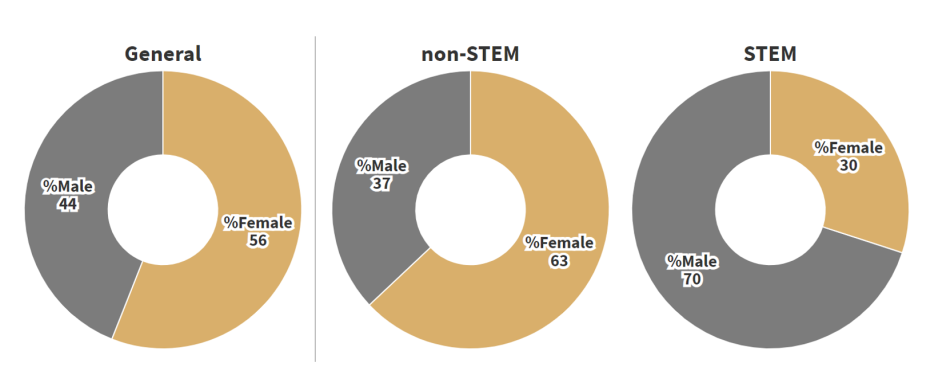
\includegraphics[width=.9\textwidth]{chaps/Images/genderpizza.png}
    \caption{Distribuição de gênero no ensino superior brasileiro}
    \label{fig:genderpizza}
\end{figure}

O projeto SAGA considera a paridade de gênero como aceitável quando varia de 45\% a 55\%. No Brasil, dos 122 cursos superiores de CTEM, apenas 13 deles estão nessa faixa aceitável de paridade de gênero. Considerando as 20 licenciaturas com maior número de alunos matriculados, apenas três delas atingiram a paridade de gênero (Tabela 1). Nesta lista dos 20 melhores cursos, podemos destacar os cursos da área de Tecnologia da Informação como os piores em termos de paridade de gênero, com percentuais de alunas variando de 16\% a uns impressionantes 8\% em Redes de Computadores.

\begin{figure}
    \centering
    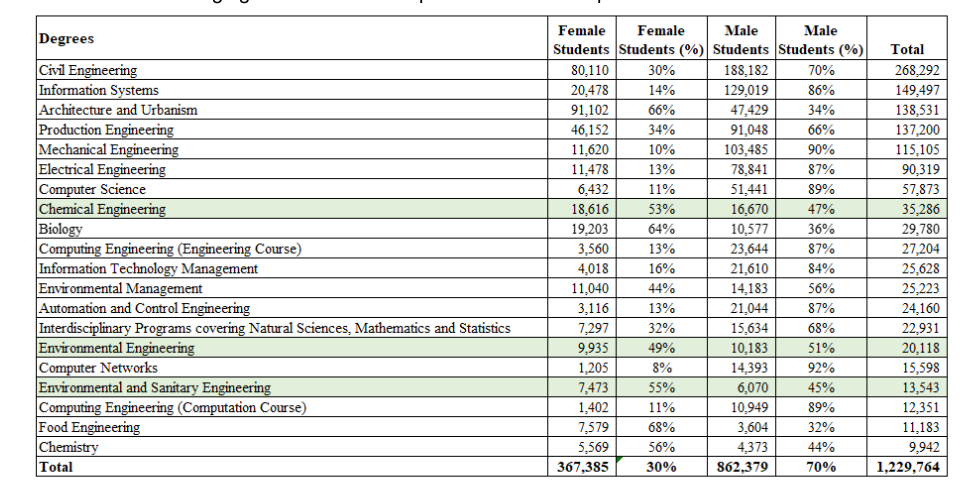
\includegraphics[width=.9\textwidth]{chaps/Images/gendertable.png}
    \caption{Matrículas de gênero no ensino superior brasileiro.}
    \label{fig:gendertable}
\end{figure}

Um dos indicadores sugeridos pela SAGA é o total de professoras por disciplina. Esse indicador é apresentado na Tabela 2 onde se pode verificar que, em termos da proporção total de docentes do sexo feminino em disciplinas relacionadas às CTEM, alcançamos a paridade de gênero no Brasil. Ainda assim, quando olhamos individualmente para as graduações, é possível ver que das 20 disciplinas, apenas quatro têm paridade de gênero com as professoras sendo significativamente sub-representadas em disciplinas como Engenharia, Computação, Física e Astronomia - todas com menos de 30\% de professoras.

\begin{figure}
    \centering
    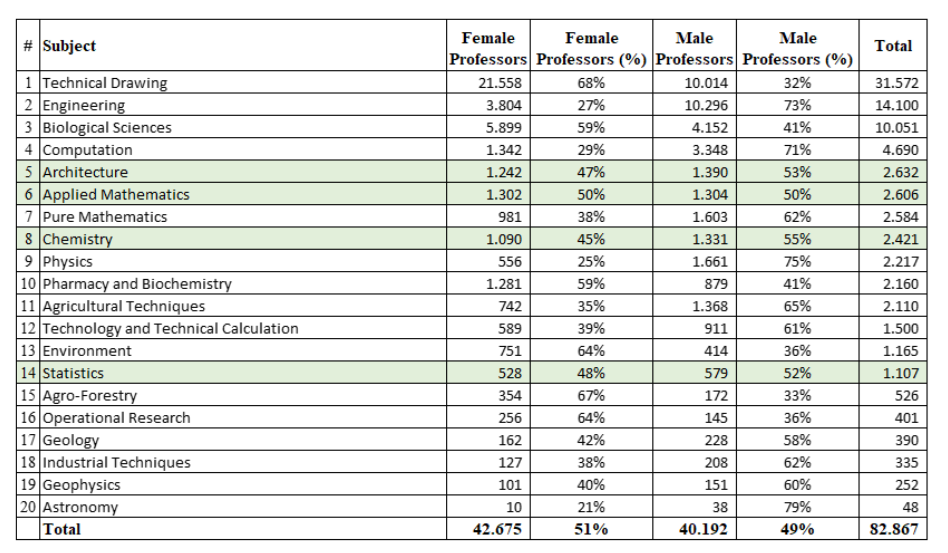
\includegraphics[width=.9\textwidth]{chaps/Images/gendertable2.png}
    \caption{Docentes por disciplina do Ensino Superior Brasileiro.}
    \label{fig:gendertable2}
\end{figure}

\subsection{Iniciativas para Igualdade de Gênero no Brasil}

A Tabela 3 apresenta os resultados de nossa pesquisa de iniciativas para aumentar a igualdade de gênero em STEM no Brasil. Os resultados são apresentados de acordo com o framework fornecido pela SAGA Policy Matrix [18]. Das 25 iniciativas apresentadas, 7 tiveram suas informações cadastradas em nosso formulário online por seus organizadores e 18 foram cadastradas pelos pesquisadores. Como se pode ver, apenas uma iniciativa é organizada pelo governo, enquanto a maioria delas são organizadas ou apoiadas por empresas e universidades. Ao se olhar para o tipo de instrumento, quase todas as iniciativas proporcionam algum tipo de formação em CTEM para mulheres e envolvem a criação e auxílio de pólos tecnológicos, centros de excelência ou comunidades. Apenas duas iniciativas, “Meninas Digitais” e “Para Mulheres na Ciência”, oferecem bolsas de estudo. Além disso, apenas duas iniciativas organizam feiras ou fornecem assistência técnica para mulheres em STEM. o
os beneficiários das iniciativas são, em todos os casos, estudantes e exclusivamente mulheres. A cobertura geográfica das iniciativas é estadual ou nacional, sendo apenas cinco delas internacionais. Os Objetivos de Gênero de Ciência e Tecnologia número 1 da SAGA Unesco se preocupam em mudar as normas sociais e os estereótipos em relação às mulheres em STEM na sociedade. Todas as iniciativas pesquisadas
estão de alguma forma contribuindo com esse objetivo. Outro objetivo da SAGA Unesco que está relacionado com quase todas as iniciativas é o objetivo número 7 que diz respeito à promoção da igualdade de género nas atividades de empreendedorismo e inovação. O objetivo número 3, a participação das mulheres no ensino superior STEM, está relacionado com 20 iniciativas. Já o objetivo menos encontrado nas iniciativas pesquisadas é o objetivo número 6, que trata da igualdade de gênero no processo de formulação de políticas. Em termos de ODS, podemos ver que, como se pode esperar, todos eles estão relacionados ao ODS 5 que se preocupa com o alcance da igualdade de gênero e empoderamento das mulheres. Além disso, 60\% das iniciativas estão de alguma forma relacionadas ao ODS 4, aquele que tem como foco a educação inclusiva e equitativa para todos. Também uma preocupação para um terço das iniciativas pesquisadas é a promoção do crescimento econômico sustentável e do emprego para todos (ODS 8).

\begin{figure}
    \centering
    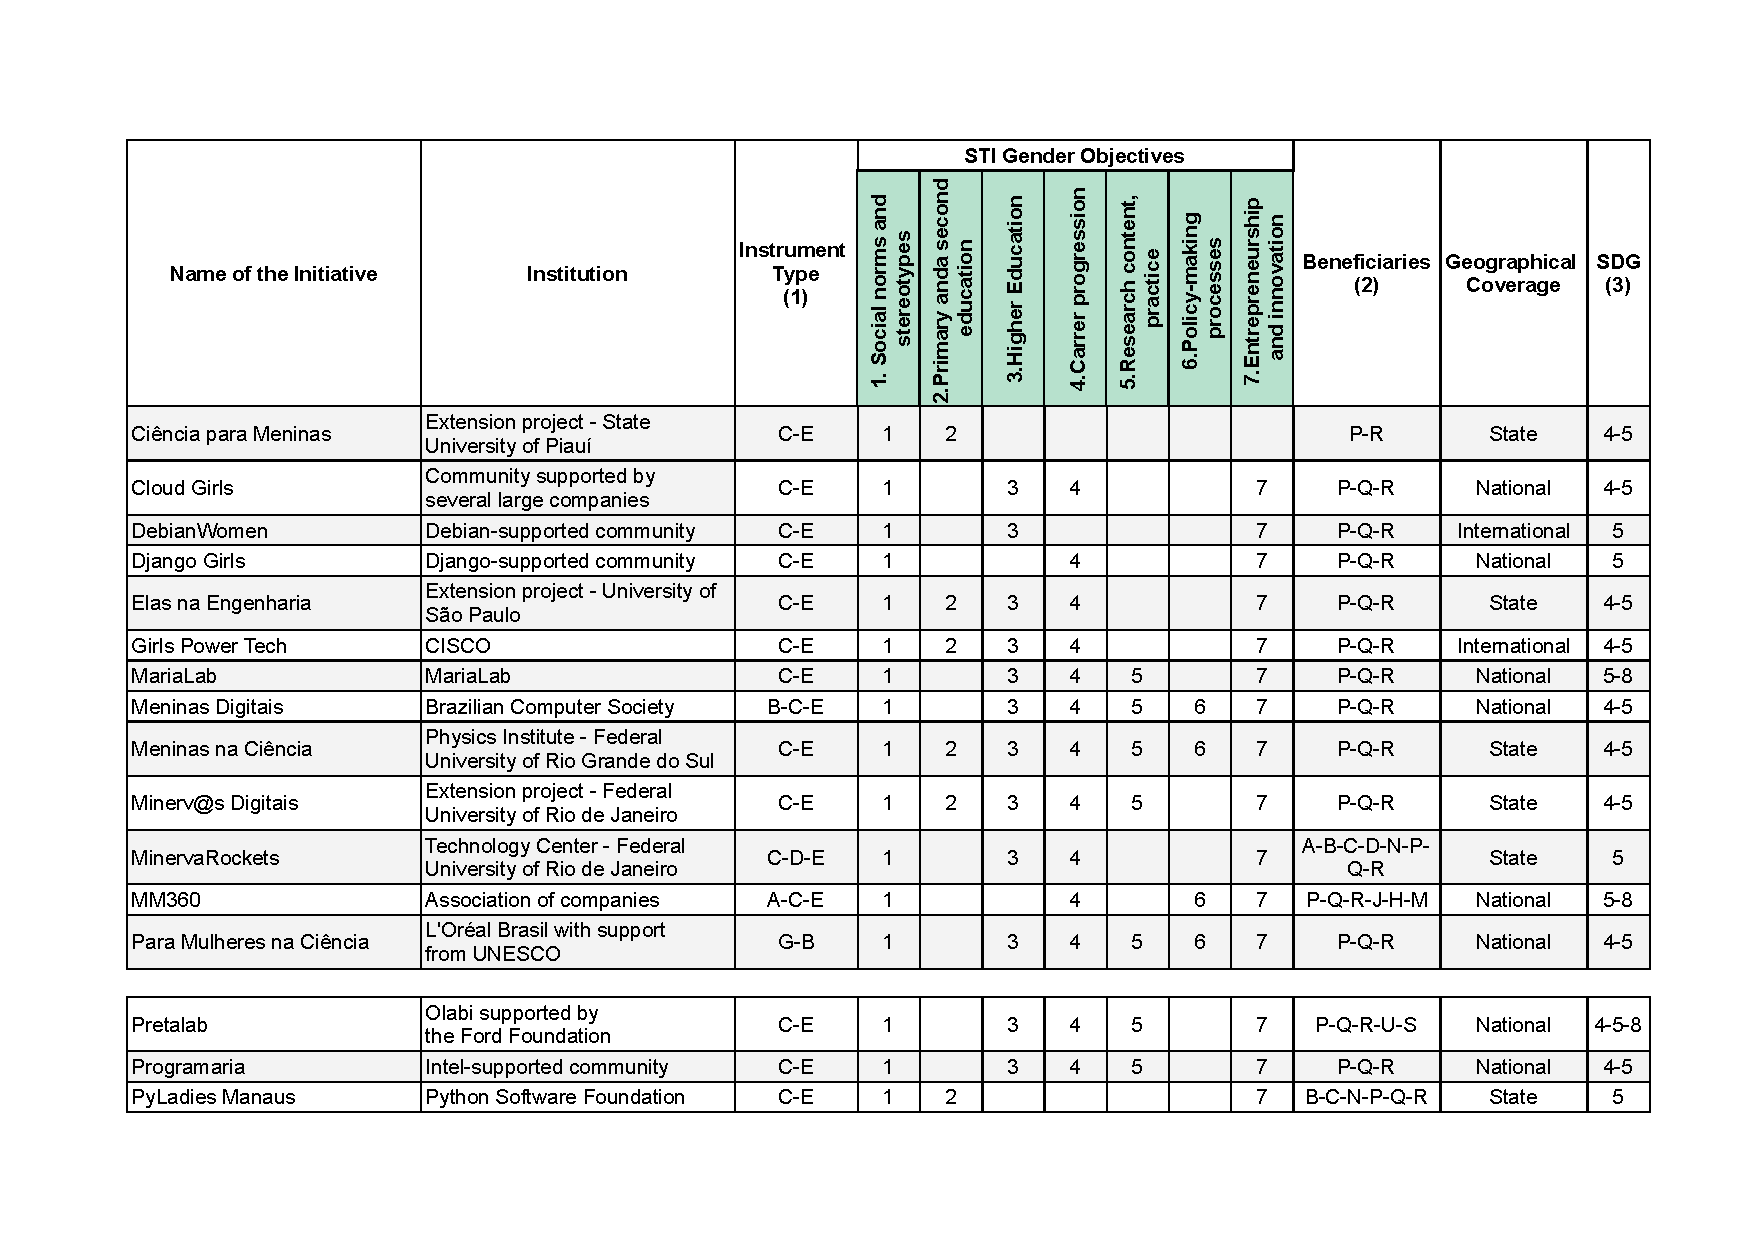
\includegraphics[width=.9\textwidth]{chaps/Images/SAGAMatrixV2.pdf}
    \caption{Iniciativas STEM para a igualdade de gênero no Brasil}
    \label{fig:sagamatriz}
\end{figure}

(1) Tipo de instrumento corresponde às seguintes categorias: A - Assistência Técnica; B - Bolsas / Bolsas de estudo; C - Treinamento; D - Prêmios e Competições; E - Criação e auxílio de pólos tecnológicos, centros de excelência e comunidades; F - Doações (pessoas físicas / jurídicas); G - Feiras; H - confiança; I - Garantia Financeira; J - Incentivos de crédito e capital de risco; K - Incentivos fiscais; L - Empréstimos; M - Serviços de Informação; N - Subsídio (contribuições não reembolsáveis).

(2) Beneficiários ”corresponde às seguintes categorias: A - Centros de pesquisa; B - Universidades; C - Escolas / Faculdades / Institutos; D - Centros de treinamento técnico; E - Institutos públicos; F - Institutos profissionais; G - Organizações STI públicas ou privadas sem fins lucrativos; H - Empresas privadas; I - Pequenas e médias empresas; J - Cooperativas; K - Fundações; L - Grupos locais de P/D; M - associações ad hoc; N - Professores e pesquisadores universitários; O - Equipe técnica e assistentes em STI; P - Alunos; Q - Indivíduos; R - Mulheres (exclusivamente); S - Povos indígenas e comunidades locais; T - Pessoas com deficiência; U - Minorias; V - Profissionais / Ph.D.s.

(3) “Objetivo de Desenvolvimento Sustentável (ODS)” corresponde aos seguintes objetivos: 4 - Garantir uma educação de qualidade inclusiva e equitativa e promover oportunidades de aprendizagem ao longo da vida para todos; 5 - Alcançar a igualdade de gênero e empoderar todas as mulheres e meninas; 8 - Promover o crescimento econômico sustentado, inclusivo e sustentável, emprego pleno e produtivo e trabalho decente para todos.

\subsection{Conclusão}

No Brasil, a Constituição Federal de 1988 garante direitos iguais para homens e mulheres, com especial destaque para o mercado de trabalho. Para que esses direitos sejam efetivamente colocados em termos de igualdade entre homens e mulheres, o caminho para a igualdade de gênero passa por um esforço que depende do governo, ONGs, instituições de ensino e empresas. Particularmente no STEM, esse caminho está sendo mostrado ainda mais difícil de seguir. Além dos desafios enfrentados atualmente pelas mulheres, como a língua predominantemente masculina em ambientes educacionais, de negócios e na cultura em geral, a pandemia COVID-19 cria novos desafios e agrava os anteriormente existentes. A atual pandemia global e o distanciamento social que exige aumentam os obstáculos às mulheres na Ciência, visto que são mais solicitadas no trabalho doméstico e no cuidado, “agravando todas as desvantagens que as mulheres já enfrentam” \citep{scientists_scientist_nodate}. Conforme os dados apresentados por este estudo mostra que existe uma grande lacuna de gênero em STEM, ainda mais em áreas de Tecnologia como Ciência da Computação. Por isso, o Brasil precisa investir em iniciativas exemplares voltadas para a promoção da igualdade de gênero em STEM, como PyLadies (das regiões de Manaus 1, Paraíba 2, Sul de Minas Gerais 3); Meninas na Ciência 4; Ciência para meninas; Elas na Engenharia 5 e Minerva Digitais 6. Essas iniciativas, como mostrado em nossa pesquisa, são importantes para atrair meninas para carreiras em ciência e tecnologia; fomentar o interesse nas áreas exatas e tecnológicas; incentivando e apoiando a participação das mulheres na área tecnológica; incentivando mais meninas e mulheres a aprender sobre a programação; ajudar mais mulheres a se tornarem atuantes em comunidades de software livre; e
incentive as meninas a seguirem carreiras em STEM. Os resultados de nosso estudo podem ser usados para comparar o caso brasileiro com outros países em termos do estado atual da igualdade de gênero no Ensino Superior STEM, bem como as iniciativas para diminuir a lacuna de gênero. O documento também pode ser usado para ajudar os interessados em desenvolver iniciativas para a igualdade de gênero em STEM a entender quais problemas eles querem ajudar a resolver, comparando seus objetivos com os levantados em nosso trabalho.




\subsection{Evento Jornada das Mulheres}

\subsection{Artigos publicados}

\subsection{Trabalhos apresentados}


\section{Motivação de Estudantes}

O conceito de motivação é essencial para a educação. \citep{howard_bell_terrell_1981}, colocou a questão de forma enfática: “Há três coisas a lembrar sobre a educação. O primeiro é a motivação. O segundo é a motivação. A terceira é a motivação ”(\citet{howard_bell_terrell_1981}. Em nosso trabalho, pretendemos identificar os comportamentos relacionados ao aluno, juntamente com um conjunto de características motivacionais, que esperamos que sejam intrínsecas. Saber que a atitude de um aluno durante ela / seu envolvimento com o conteúdo de aprendizagem, dentro ou fora da sala de aula, envolve um relacionamento complexo com várias pessoas, como professores, colegas e equipe, nosso objetivo é envolver o maior número possível de stakeholders no processo de aprendizagem.

\subsection{Teoria da Autodeterminação}

De acordo com \citet{ryan_self-determination_2000}, existem dois aspectos dominantes que podem ser identificados na determinação da motivação: motivação extrínseca e intrínseca.

A motivação intrínseca surgiu na década de 1950 com experimentos em macacos \citet{harlow_learning_1950}. Os primeiros experimentos com humanos foram realizados na década de 1970 \citep{deci_effects_1971} e na década de 1980 aspectos como feedback, prazos e vigilância de motivações intrínsecas foram examinados \citep{deci_intrinsic_1985}.

Com base no conceito anterior de motivação intrínseca, \citet{ryan_self-determination_2017} propôs a Teoria da Autodeterminação (SDT) `` uma teoria organísmica baseada empiricamente do comportamento humano e desenvolvimento da personalidade '' \citep{ryan_self-determination_2017}.

Entre suas características, competência e autonomia, junto com o parentesco, são os principais elementos trabalhados na SDT. Uma vez que os humanos tenham essas necessidades atendidas, a motivação intrínseca pode surgir, e quando elas não são atendidas, a motivação intrínseca é danificada \citet{ryan_self-determination_2017}.

Além disso, essa motivação intrínseca está associada à busca por novidades e desafios, com o intuito de explorar e aprender \citep{ryan_self-determination_2000}, que pode gerar criatividade, desempenho em atividades e uma experiência efetiva \citep{di_domenico_emerging_2017}.

A motivação intrínseca é a forma mais importante de motivação no desempenho do ensino médio  \citep{taylor_self-determination_2014,froiland_intrinsic_2016}, com resultados positivos também no ensino superior  \citep{williams_importance_1998, muller_continuity_2005}, pesquisas incluindo ensino superior e STEM \citep{de_loof_teachers_2019, wang_multilevel_2020} e incluindo ensino superior, STEM e mulheres \citep{moore_connecting_2020, skewes_absent_2018}.

\citep{chua_association_2021} afirma que `` No SDT, o progresso de nosso objetivo é influenciado não apenas pelo que fazemos, mas também pelo que recebemos ". Alguns autores estudam a importância dos objetivos e sua relação com o desempenho dos alunos no contexto da educação \citet{chua_association_2021, benita_emotion_2021, benita_important_2017, benita_when_2014}.

Atualmente, os ambientes de aprendizagem online são importantes mecanismos digitais de atratividade para os alunos, sendo também objetos de pesquisa com a aplicação do SDT \citet{chiu_applying_2021, chiu_digital_2021, chen_motivation_2010}

\subsection{Teoria da Metas}

\section{Autorregulação da Aprendizagem}

\subsection{Mapeamento Sistemático de Autorregulação da Aprendizagem}

Esta seção discute como quizzes são aplicados no campo do aprendizado da engenharia de software e como os quizzes podem ajudar a autorregular o aprendizado do aluno. Para isso, foi realizado um mapeamento sistemático que selecionou os estudos mais relevantes sobre o uso de quizzes na educação, com o objetivo de esclarecer suas relações e impactos mútuos. Nossa análise mostra que o envolvimento do aluno e o trabalho com quizzes são soluções de aprendizagem proeminentes para aumentar a motivação dentro e fora da sala de aula. Argumentamos que compartilhar os quizzes aumentará o potencial para que eles sejam usados como uma ferramenta de autorregulação no ensino de engenharia de software. 

\subsection{Introdução}

A forma de aprendizagem do aluno muda, principalmente com o uso de ferramentas tecnológicas \cite{nilson_creating_2013, fink_creating_2013, ebert_school_2013}. Apesar disso, os tipos de aprendizagem ativa têm como objetivo principal colocar o aluno no centro do processo de aprendizagem e não necessariamente focado no uso da tecnologia. Exemplos disso ocorrem até mesmo nas abordagens utilizadas desde a época de Aristóteles (384 aC-322 aC) \cite{berge_computer_1995}, como uma aula onde os alunos ficam sentados em uma roda, discutindo e refletindo, entre todos, um assunto específico.

Um dos elementos tecnológicos utilizados como recurso de aprendizagem são os quizzes. O uso de quizzes para aprendizagem existem há muitos anos desde que foi discutido pela primeira vez \cite{mawhinney_comparison_1971}. Os quizzes têm sido usados no ensino médio, como uma ferramenta de avaliação e para apoiar outros métodos ou técnicas educacionais em vários campos diferentes, incluindo cursos de engenharia \cite{herold_student_2012, thevathayan_imparting_2017, figueiredo_evaluation_2014}. 

Grimstad \cite {grimstad_are_2004} encontrou resultados que indicam que os alunos podem usar quizzes para melhorar seu desempenho no exame. Para que essa melhoria de desempenho ocorra, Bangert-Drowns \cite {bangert-drowns_instructional_1991} analisou que o feedback está relacionado à aprendizagem e concluiu que os alunos aprendem mais se receberem a resposta correta somente após responder a uma pergunta. Também descobriu que o feedback corretivo é melhor do que simplesmente dizer aos alunos que eles estavam certos ou errados, o que significa que é importante orientar o aluno para as áreas de conteúdo onde ele precisa de revisão ou estudo adicional. Isso se deve ao fato de que, segundo o autor, promove uma estratégia com aspectos de preparação, execução, feedback e autorreflexão.

Para melhor esclarecer o estado atual da pesquisa, envolvendo a utilização de quizzes, na educação e, principalmente, no ensino de Engenharia de Software, realizamos um mapeamento sistemático. Este mapeamento tem como objetivo principal construir uma base de conhecimento que permita explorar quizzes, como ferramenta de aprendizagem autorregulada, no ensino de Engenharia de Software.

Para isso, nosso estudo apresenta as seguintes questões de pesquisa:

\begin {itemize}
    \item\textbf {RQ $ _1 $ - Os quizzes são usados no ensino de engenharia de software?}
     \item\textbf {RQ $ _2 $ - Como os quizzes são usados no ensino de engenharia de software?}
     \item\textbf {RQ $ _3 $ - Os quizzes são usados na educação em engenharia de software para a autorregulação da aprendizagem?}
     \item\textbf {RQ $ _4 $ - Como a aplicação de Quizzes no Ensino de Engenharia de Software pode ser utilizada na Autorregulação da Aprendizagem?}
     \item\textbf {RQ $ _5 $ - Como podemos melhorar o uso de Quizzes no Ensino de Engenharia de Software?}
\end {itemize}

Para responder a essas perguntas, realizamos uma revisão de mapeamento em cinco seções, começando com a introdução (seção 1) e, em seguida, progredindo da seguinte forma: a seção 2 apresenta uma breve revisão dos questionários; A seção 3 inclui os conceitos e metodologia usados neste trabalho; a seção 4 cobre os resultados e nossa análise de pesquisa; E finalmente, na seção 5, nossas conclusões são apresentadas.

\subsection{Educação e Quizzes}

Anderson \cite{anderson_reflections_1984} discutiu e analisou questões sobre processos educacionais. Esses processos incluíam fontes de motivação, como crenças de autoeficácia, gratificação atrasada, atribuições, valores e interesses. Bem como fontes de metacognição como estabelecimento de metas, uso de estratégia, automonitoramento e autoavaliação.

Recentemente, devido aos mais recentes desenvolvimentos em recursos tecnológicos, métodos, dinâmicas e elementos motivacionais, a educação tem transformado os métodos tradicionais de ensino em novos conceitos de aprendizagem, como a sala de aula invertida e a aprendizagem autorregulada.

A sala de aula invertida é uma pedagogia baseada em tecnologia. Bishop e Verleger\cite {bishop_flipped_2013} definem este tipo de aprendizagem como uma instrução individual direta, baseada em computador, fora da sala de aula. Além disso, segundo os autores, esse processo também é realizado por meio de vídeo-aulas e atividades interativas de aprendizagem em grupo em sala de aula.

Como resultado de todas essas transformações na educação, a visão atual da tarefa do aluno na educação mudou para descobrir como aprender novos conhecimentos, em vez de criar verdades e conhecimentos únicos \cite{ebert_school_2013}. Ao refletir sobre suas ações e como encontrar novos conhecimentos, o aluno pode descobrir por si mesmo como superar seus próprios desafios.

Berge\cite{berge_computer_1995} compara a prática da sala de aula invertida com a abordagem baseada no diálogo praticada na Grécia antiga, onde as pessoas aprendiam por meio de desafios e atividades da vida real, compartilhando seus próprios pensamentos e opiniões a fim de encontrar soluções para seus problemas.

Zimmerman e Risemberg \cite{zimmerman_chapter_1997} explicaram as implicações dos diferentes componentes da aprendizagem autorregulada, ressaltando que as tarefas propostas devem permitir que os alunos tomem decisões pessoais e ponderadas com o intuito de regular seus processos de aprendizagem. Com base nessas implicações, o modelo cíclico de Zimmerman \cite{zimmerman_chapter_2000} foi estabelecido (uma representação esquemática está incluída na Fig.\Ref {fig:Zimmerman Model}). De acordo com Zimmerman, a aprendizagem autorregulada visa definir o processo de aprendizagem e as crenças motivacionais de um aluno com base em três fases de autorregulação: Forethought, Performance e Self-Reflection \cite {zimmerman_investigating_2008}.

\begin{figure}[!t]
\centering
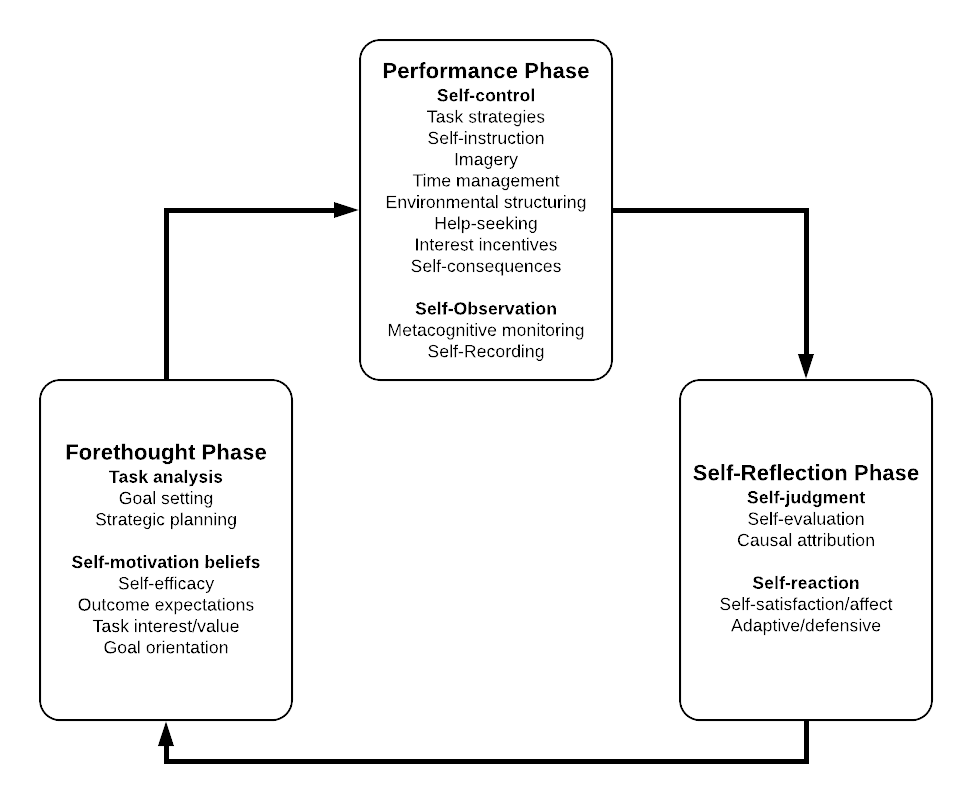
\includegraphics[width=3.5in]{chaps/Images/Zimmerman.png}
\caption{Zimmerman Cyclic Model.}
\label{fig:Zimmerman Model}
\end{figure}

A aprendizagem autorregulada também foi considerada importante nas formas sociais de aprendizagem, como buscar ajuda externa de outras pessoas que não o professor. A questão principal é se o aluno demonstra iniciativa pessoal e capacidade de adaptação. Essas qualidades dos alunos derivam de crenças e sentimentos motivacionais vantajosos \cite{zimmerman_chapter_2000}.

De acordo com Anderson et al. \cite{anderson_taxonomy_2000}, existem dois tipos de avaliação. O primeiro tipo é a avaliação somativa, em que as informações são coletadas pós-aprendizagem para determinar o quão bem o aluno aprendeu o material. O outro tipo é a avaliação formativa, que se preocupa com a coleta de informações sobre o aprendizado e é projetada para melhorar a qualidade ou a quantidade do aprendizado.

Os quizzes são normalmente usados para fazer os testes de avaliação de conhecimentos e habilidades de um aluno. Os quizzes não devem ser entendidos apenas como avaliações sumativas, mas sim como uma experiência de aprendizagem para os alunos, avaliando a eficácia das suas estratégias de estudo e preparação para o teste \cite{nilson_creating_2013}. Como tal, são um dos elementos que podem ser aplicados na educação para melhorar a aprendizagem autorregulada.

É importante considerar que aprender a usar o material de estudo é tão importante quanto aprender o próprio material. Desta forma os alunos irão avaliar suas estratégias e se preocupar com seu desempenho, aprimorando-as adequadamente \cite{fink_creating_2013}. Para tanto, Zimmerman sugere que os alunos devem primeiro ser solicitados a expressar sua confiança na capacidade de resolver um problema antes de começarem a tentar resolvê-lo e reavaliar sua confiança após resolvê-lo. Depois disso, eles devem ser solicitados a escrever uma análise de erros de todos os problemas que eles não resolveram corretamente. Ao fazer a primeira atividade, os alunos aprendem rapidamente a estudar um problema antes de tentar resolvê-lo; enquanto faz o segundo, permite que eles adquiram estratégias de solução de aprendizagem \cite{zimmerman_enhancing_2011}.

Ottenhoff \cite{ottenhoff_learning_2011} afirma que a literatura sobre aprendizagem autorregulada, metacognição e avaliação oferece várias atividades e tarefas que os alunos podem realizar antes, durante e depois dos exames. Algumas atividades e atribuições tornam os alunos mais conscientes do que aprenderam e não aprenderam, enquanto outras atividades envolvem os alunos na avaliação de estratégias de preparação para o teste e no desenvolvimento de estratégias mais eficazes. Todos eles ajudam a melhorar o foco dos alunos em seu aprendizado. De acordo com Nilson \cite{nilson_creating_2013}, os quizzes podem apoiar a aprendizagem autorregulada, fornecendo oportunidades para várias Atividades e Tarefas que ajudam na aprendizagem autorregulada. Incluem Atividades e Tarefas para Preparação para Exames, Atividades Durante um Exame e Atividades e Tarefas Após Exames e Testes.

Antes dos exames, os alunos podem se preparar estudando e melhorando suas áreas de conhecimento mais fracas, mas existem opções que consomem menos tempo. Ao criar perguntas de teste desenvolvidas pelos alunos (de múltipla escolha ou outros tipos de perguntas), os alunos podem revisar o material e avaliar a importância de diferentes partes do material. A criação de uma Folha de Revisão Criada pelo Aluno que mapeia as principais áreas de conteúdo permite ao aluno estimar a porcentagem do exame que será composta por essa área. Esta folha de revisão pode ser melhorada listando o que os alunos acreditam que eles deveriam ser capazes de fazer ou demonstrar e usar esta folha de revisão para se preparar. Os alunos podem elaborar Pesquisas de Conhecimento Pré-exame (quizzes que lhes pedem para avaliar sua confiança em sua capacidade de responder a perguntas ou realizar tarefas relacionadas ao curso). Isso familiariza os alunos com o objetivo do quiz/exame e revela o conteúdo e as áreas de habilidade nas quais eles são fracos ou fortes, permitindo-lhes estreitar o foco de seu estudo e incentivando o estabelecimento de metas e o autoteste.

Durante um exame, os alunos podem ser solicitados a avaliar sua confiança em sua capacidade de resolver um problema antes e depois de resolvê-lo. Incorporar uma pesquisa de conhecimento em um exame pode permitir que os resultados sejam avaliados pela confiança do aluno neles.

Após um Exame, existem várias oportunidades de aprendizagem autorregulada. Pode-se pedir aos alunos que reflitam sobre o quanto estavam preparados para um quiz e sobre a eficácia de seu método de preparação, permitindo-lhes revisar e reconsiderar seus métodos de preparação e capacidade atual. A devolução de um quiz com notas oferece a oportunidade para os alunos resolverem problemas que perderam anteriormente ou resolverem problemas semelhantes. Se isso for combinado com a autoavaliação pré-questionário ou pré-exame de seus níveis de confiança e da eficácia de seu método de estudo, permite saltos impressionantes no aprendizado do aluno. Os alunos podem responder a perguntas no final de um exame para estimar seu desempenho, para descrever sua preparação e para avaliar a dificuldade em diferentes partes do exame. Isso faz com que os alunos reflitam e prevejam seu desempenho, avaliem sua preparação e a eficácia de seus métodos de preparação, reavaliem sua confiança após receberem o exame com notas e vejam se suas estratégias de preparação estão funcionando. A formalização da reavaliação dos métodos e da confiança de um aluno é possível fazendo com que os alunos respondam por escrito a uma série de perguntas depois de verem seu exame com nota, permitindo assim que os alunos desenvolvam um plano de estudo para o próximo exame com base nos resultados do exame anterior. Usando a análise pós-teste, os alunos são capazes de diagnosticar os padrões por trás de seus erros e, assim, obter o tipo de ajuda de que precisam.

Embora existam muitas questões teóricas e práticas sobre como maximizar os benefícios do uso dos quizzes, interromper o aprendizado com perguntas do questionário é benéfico porque pode melhorar o envolvimento do aluno \cite{healy_timing_2017}. Diversas instituições de ensino adotam clickers, que permitem aos instrutores aplicar questionários de múltipla escolha a qualquer momento durante a aula, com feedback imediato para professores e alunos \cite{smith_why_2009}. De acordo com Harley, há um benefício de aprendizagem para os alunos, proporcionado pela ação de testar seus conhecimentos, pela obtenção de feedback e pela natureza interativa do procedimento do clicker. Para os professores, há o benefício da avaliação por ter a capacidade de manter uma avaliação contínua da compreensão dos alunos e prever sua retenção de aprendizagem após a leitura do material \cite{healy_timing_2017}.

Com o entendimento de que os quizzes podem ser aplicados à educação, apesar do aparente desafio e sobrecarga necessários para preparar e administrar questionários em um contexto educacional, este estudo tem como objetivo investigar como os quizzes podem ser benéficos para a aprendizagem autorregulada, no contexto das aulas de engenharia de software.

\subsection{Metodologia}
\label{metodo}

O processo de pesquisa utilizado neste trabalho baseia-se na revisão sistemática da pesquisa de processos em engenharia de software \cite{kitchenham_systematic_2013, kitchenham_systematic_2009} e foi conduzida por meio da plataforma Parsif.al \footnote{https://parsif.al/}.

Nosso processo começou com um mapeamento sistemático que nos permite avaliar e selecionar os estudos mais relevantes sobre o uso de quizzes para auxiliar na autorregulação da aprendizagem. Nossa intenção é identificar a utilização de quizzes na autorregulação da aprendizagem no contexto de alunos de graduação, no ensino de engenharia de software.

Exploramos como o ensino de engenharia de software utiliza quizzes, quais são seus tipos, se é utilizado como ferramenta de autorregulação da aprendizagem e quais resultados positivos e negativos foram encontrados. Para nós, é importante entender como eles podem ser usados de diferentes maneiras. Todos os procedimentos de revisão da literatura - como descrição do que foi planejado, seleção da estratégia, condução da pesquisa e relatório final - são descritos a seguir.

\subsection{Research Planning}
\label{planeja}

Nosso plano de pesquisa foi elaborado contendo: objetivos, questões a responder, busca e seleção, estratégias, avaliação da qualidade e extração de resultados. Nosso planejamento de pesquisa começou com a definição do protocolo para o mapeamento sistemático. Começamos definindo os objetivos de nossa pesquisa:
\begin{itemize}
     \item Analisar publicações científicas que abordem o Ensino de Engenharia de Software;
     \item Analisar publicações científicas que estudam a utilização de Quizzes no Ensino (e em particular como ferramenta pedagógica autorreguladora);
     \item Elaborar uma Revisão e/ou Mapeamento da literatura sobre `` Ensino e Questionários de Engenharia de Software '';
     \item Justificar/motivar a criação/implementação de um repositório de Quiz Compartilhado de Engenharia de Software
\end{itemize}

Nossa próxima etapa foi definir a População, Intervenção, Comparação, Resultado, Contexto (PICOC):
\begin{itemize}
     \item População - `` questionários "
     \item Intervenção - autorregulação da aprendizagem
     \item Comparação - iniciativa OU modelo OU estrutura OU atividades OU métodos OU técnicas
     \item Resultado - apoiar OU melhorar OU otimizar OU ajudar OU ajudar OU especificações
     \item Contexto - Educação em Engenharia de Software
\end{itemize}

Em seguida, definiu-se as questões de pesquisa:
\begin{itemize}
    \item\textbf{RQ $ _1 $ - Os questionários são usados no ensino de engenharia de software?} - O objetivo desta questão é verificar se os questionários são usados como ferramenta de aprendizagem no ensino de engenharia de software.
    
\item\textbf{RQ $ _2 $ - Como os Quizzes são usados no Ensino de Engenharia de Software?} - O objetivo desta questão é entender quais tipos de quizzes foram aplicados e como eles foram usados no Ensino de Engenharia de Software.

\item\textbf{RQ $ _3 $ - Os questionários são usados na Educação em Engenharia de Software para a Autorregulação da Aprendizagem?} - O objetivo desta questão é entender quais áreas de pesquisa, relacionadas à autorregulação da aprendizagem, foram afetadas pelo uso de questionários.

\item\textbf{RQ $ _4 $ - Como a aplicação de Quizzes na Educação em Engenharia de Software pode ser utilizada na Autorregulação da Aprendizagem?} - Esta questão busca identificar quais etapas da autorregulação da aprendizagem, com base no modelo cíclico de Zimmerman, foram aplicados, seus resultados e suas falhas de implementação.

\item\textbf{RQ $ _3 $ - Como podemos melhorar o uso de questionários no ensino de engenharia de software?} - Esta questão busca identificar possíveis melhorias no uso atual de questionários no ensino de engenharia de software.
\end{itemize}.

Em relação às palavras-chave e sinônimos, selecionamos as seguintes palavras-chave, mas optamos por não definir nenhum sinônimo para evitar a obtenção de resultados que escapassem ao escopo deste trabalho:

\begin{itemize}
     \item Quiz
     \item Aprendizagem de Autorregulação
     \item Educação em Engenharia de Software
\end{itemize}

Escolhemos o banco de dados de estudos Scopus \footnote{http://www.scopus.com} como nossa fonte. Para a busca de artigos, utilizamos artigos dos últimos 5 anos em nossas fontes selecionadas. Definimos a seguinte string de pesquisa \emph{`` quiz "AND` `Educação em Engenharia de Software"}.

Definimos vários critérios de inclusão e exclusão para que pudéssemos aceitar ou rejeitar os estudos que obtivemos em nossa busca. Estes são mostrados em \textbf{Tabela\ref{tab:criteria}}.

\begin{table}[ht]
    \centering
        \caption{Critérios de inclusão e exclusão para estudos}
        \begin{tabular}{p{65mm}|p{65mm}}
            \hline
                \textbf{Critérios de inclusão} & \textbf{Critérios de exclusão} \\
            \hline
            \hline
                O estudo apresenta métodos e técnicas possíveis & O estudo aborda questionários fora do contexto da engenharia de software 
                \\
            \hline
                O estudo apresenta possíveis implicações (vantagens e desvantagens)  &
                O estudo é um capítulo de um livro ou editorial \\
            \hline
                O estudo apresenta questões relacionadas à nossa pesquisa  &
                O estudo não está disponível para leitura \\
            \hline
                 - &
                O estudo não está relacionado às questões de pesquisa \\
            \hline
                 - &
                O estudo não foi publicado em inglês \\
            \hline
        \end{tabular}
    \label{tab:criteria}
\end{table}

Após finalizar a definição do protocolo, definimos uma Lista de Verificação de Avaliação da Qualidade que nos permitiu avaliar a qualidade de cada um dos estudos aceitos.

A lista de verificação foi composta por duas questões que consideramos adequadas aos objetivos de nossa pesquisa:

\begin {itemize}
     \item No artigo foram encontrados - Auto-regulação da aprendizagem - afetada pelo uso de quizzes?
     \item No artigo foram encontrados - tipos de quizzes - aplicados no ensino de engenharia de software?
\end{itemize}

Definimos três respostas para as questões e seus respectivos pesos. Eles são mostrados em \textbf {Tabela\ref{tab:scoring_weight}}.

\begin{table}[ht]
    \centering
        \caption{Respostas da pergunta da lista de verificação de avaliação de qualidade e respectivo peso}
        \begin{tabular}{c|c}
            \hline
                \textbf{Responder} & \textbf{Peso} \\
            \hline
            \hline
                Sim & 2.0 \\
            \hline
                Parcial & 1.0 \\
            \hline
                Não & 0.0 \\
            \hline
        \end{tabular}
    \label{tab:scoring_weight}
\end{table}

A pontuação máxima foi calculada automaticamente (4,0) e optamos por um Cutoff Score (que nos permite descartar qualquer estudo que ficasse abaixo da pontuação escolhida) de 3,0.

Para que pudéssemos sistematizar a extração dos dados dos estudos, criamos um Formulário de Extração de Dados que nos ajudaria a encontrar as respostas às nossas dúvidas de pesquisa nos seguintes campos:

\begin{itemize}
    \item \textbf{Tipo de Aplicação de Quizzes} - O objetivo deste campo é extrair dados sobre como os questionários foram aplicados à Engenharia de Software (tipos de questionários). Nos permite responder \textbf{RQ$_1$ - Os quizzes são usados no ensino de engenharia de software?} e \textbf{RQ$_2$ -  Como os quizzes são usados na educação em engenharia de software?}.
    
    \item \textbf{Contexto onde os quizzes foram aplicados} - O objetivo deste campo é extrair dados sobre o contexto onde os quizzes foram aplicados (a que tipo de curso ou sistema os questionários foram aplicados e quando foram aplicados). Isso nos ajudará a encontrar respostas para \textbf{RQ$_1$ - Os quizzes são usados no ensino de engenharia de software?} e \textbf{RQ$_2$ -  Como os quizzes são usados na educação em engenharia de software?}.
    
    \item \textbf{Fases do modelo cíclico de Zimmerman consideradas implícita ou explicitamente} - O objetivo deste campo é extrair dados sobre quais fases do Modelo Cíclico de Zimmerman foram envolvidas ou consideradas no estudo devido à aplicação de questionários. Isso nos ajudará a encontrar respostas para \textbf{RQ$_3$ -  Os quizzes são usados na Educação em Engenharia de Software para a Autorregulação da Aprendizagem?} and \textbf{RQ$_4$ -  Como a aplicação de Quizzes no Ensino de Engenharia de Software pode ser utilizada na Autorregulação da Aprendizagem?}.

    \item\textbf{Tipos de Atividades (Antes, Durante ou Depois do Exame/Questionário) considerada implícita ou explicitamente} - O objetivo deste campo é extrair dados sobre quais tipos de Atividades foram envolvidas ou examinadas no estudo devido à aplicação de questionários. Como o campo anterior, ele nos ajudará a encontrar respostas para \textbf{RQ$_3$ -  Os quizzes são usados na Educação em Engenharia de Software para a Autorregulação da Aprendizagem?} e \textbf{RQ$_4$ -  Como a aplicação de Quizzes no Ensino de Engenharia de Software pode ser utilizada na Autorregulação da Aprendizagem?}.
    
    \item\textbf{Resultados positivos da aplicação de questionários} - O objetivo deste campo é extrair dados sobre quais foram os resultados positivos da aplicação dos Quizzes encontrados pelo estudo. Seremos capazes de olhar para os aspectos positivos da aplicação de quizzes em engenharia de software que podem nos ajudar a raciocinar sobre \textbf{RQ$_5$ -  Como podemos melhorar o uso de quizzes na educação em engenharia de software?}.
    
    \item\textbf{Resultados negativos da aplicação de questionários} -O objetivo deste campo é extrair dados sobre quais foram os resultados negativos da aplicação dos Quizzes encontrados pelo estudo. Por estarmos cientes dos aspectos negativos, podemos tentar minimizá-los para responder \textbf{RQ$_5$ -  Como podemos melhorar o uso de quizzes na educação em engenharia de software?}.
\end{itemize}.

\subsection{Conduzindo a Pesquisa}

A seleção dos estudos utilizou um procedimento de filtragem em duas etapas: a primeira etapa envolveu a leitura dos estudos e filtrá-los de acordo com se um estudo individual está relacionado à nossa pesquisa; enquanto a segunda etapa envolveu um sistema de pontuação, em que os estudos pré-selecionados da etapa anterior foram analisados detalhadamente para determinar o grau de resposta à pesquisa (ou seja: total, parcialmente ou não todos). Em seguida, a extração foi realizada consolidando as informações relevantes contidas nos estudos. Por fim, foi realizada uma análise do resultado da etapa anterior para que pudéssemos responder às questões de pesquisa.

A pesquisa que conduzimos teve as seguintes etapas em ordem:
\begin{enumerate}

    \item \emph{Search} - Nesta etapa, pesquisamos os repositórios selecionados para a string de pesquisa definida anteriormente. Isso nos permite obter uma lista de estudos que correspondem à nossa string de pesquisa, que usaremos na próxima etapa.

    \item \emph{Import Studies} - Esta etapa permite importar as meta-informações dos estudos (resumo, autores, data, etc.) para manter um banco de dados para gerenciar as próximas etapas.

    \item \emph{Study Selection} - Durante esta etapa, aceitamos ou rejeitamos os estudos em nosso banco de dados de acordo com os critérios que definimos durante o planejamento.

    \item \emph{Quality Assessment} - Aqui, aplicamos a Lista de Verificação de Avaliação de Qualidade previamente definida aos estudos de nosso banco de dados que foram aceitos na etapa de Seleção de Estudos para pontuá-los individualmente.

    \item \emph{Data Extraction} - Usamos o Formulário de Extração de Dados criado anteriormente para extrair os dados relevantes para nossa pesquisa dos estudos em nosso banco de dados que pontuaram acima de 3,0 na etapa anterior.
    

    \item \emph{Data Analysis} - Analisamos os dados que resultaram da aplicação de nossa metodologia de pesquisa.
\end{enumerate}

\subsection{Resultados}

Nesta seção, os resultados da revisão são apresentados e analisados.

\subsection{Search}
A execução de nossa consulta de pesquisa retornou um total de 68 estudos, dos quais tínhamos 0 duplicatas.

\subsection{Study Selection}
Nossa análise dos estudos obtidos durante a Pesquisa nos fez rejeitar 46 estudos porque eles não eram relevantes para as nossas questões de pesquisa.

\subsection{Quality Assessment}
Em seguida, pontuamos os 22 estudos restantes usando a Lista de verificação de avaliação de qualidade definida anteriormente, o que resultou na manutenção dos 13 estudos. Uma visão geral dos resultados pode ser mostrada em \textbf{Table\ref{tab:quality_assessment}}.

\begin{table}[ht]
    \centering
        \caption{Visão geral das pontuações de avaliação da qualidade dos estudos}
        \begin{tabular}{c|c}
            \hline
                \textbf{Score} & \textbf{Número de estudos} \\
            \hline
            \hline
                0 & 
                1 \\
            \hline
                1 & 
                2 \\
            \hline
                2 & 
                6 \\
            \hline
                3 & 
                1 \\
            \hline
                4 & 
                12 \\
            \hline
        \end{tabular}
    \label{tab:quality_assessment}
\end{table}

\subsection{Data Extraction}

Em nossa revisão, obtivemos informações relevantes sobre quizzes em cursos de engenharia de software \cite{figueiredo_evaluation_2014}, bem como revisões sistemáticas de trabalhos que aplicaram questionários neste contexto educacional, tais como \cite{luxton-reilly_introductory_2018} e \cite {crow_intelligent_2018} . Também encontramos estudos que avaliam resultados em um ambiente de sala de aula invertida que trabalha com aprendizagem autorregulada, como \cite{ogawa_evaluation_2018} e \cite{herold_student_2012}. Práticas de aprendizagem dos alunos, como \cite{thevathayan_imparting_2017} e \cite{verdu_distributed_2012}. Um desses estudos, \cite{wu_improvement_2011} apresentou uma proposta para um conceito de jogo de aula que pode melhorar a comunicação e motivar os alunos por meio de aulas mais interessantes e sem descrever claramente como os alunos podem melhorar sua autorregulação da aprendizagem em sala de aula, este estudo pode fornecer questões importantes sobre a motivação dos alunos para autorregulação da aprendizagem  e o interesse pelo jogo, neste caso um jogo de perguntas multiplayer chamado Lecture Quiz.

\textbf{Table \ref{tab:quizzes_application_types}} mostra os dados extraídos relacionados ao \textbf{Tipo de Aplicação de Quizzes}.

\begin{table}[ht]
    \centering
        \caption{Tipos de aplicação de quizzes}
        \begin{tabular}{c|c|c}
            \hline
                \textbf{Tipos de aplicação de quizzes} & \textbf{Número de Estudos}  & \textbf{Estudos} \\
            \hline
            \hline
                Quiz Games & 
                4 &
                \cite{petri_quality_2017, petri_games_2018, verdu_distributed_2012, wu_improvement_2011} \\
            \hline
                Online Quizzes & 
                4 & 
                \cite{figueiredo_evaluation_2014, coore_facilitating_2019, luxton-reilly_introductory_2018, krugel_computational_2017} \\
            \hline
                Pop-Quizzes & 
                1 &
                \cite{luxton-reilly_introductory_2018} \\
            \hline
                Gamified Quizzes & 
                1 & 
                \cite{luxton-reilly_introductory_2018} \\
            \hline
                Quiz Creation & 
                1 & 
                \cite{ogawa_evaluation_2018} \\
            \hline
                Generic Quizzes & 
                5 & 
                \cite{crow_intelligent_2018, ogawa_evaluation_2018, acharya_infusing_2017, thevathayan_imparting_2017, herold_student_2012} \\
            \hline
        \end{tabular}
    \label{tab:quizzes_application_types}
\end{table}

Encontramos uma variedade de \textbf{Contextos onde os quizzes foram aplicados}. Separamos esses contextos nas seguintes categorias: \textbf{In-Lecture vs Outside-Lecture} e \textbf{Tipo de Curso} (Tradicional, Online, Híbrido ou Sistema Tutor Inteligente). \textbf{Tabela\ref{tab:context_in_vs_out}} mostra os contextos \textbf {In-Lecture vs Outside-Lecture} que foram encontrados para a aplicação de questionários.

\begin{table}[ht]
    \centering
        \caption{Contextos em que os quizzes foram aplicados: na aula x fora da aula}
        \begin{tabular}{c|c|c}
            \hline
                \textbf{In-Lecture vs Outside-Lecture} & \textbf{Number of Studies}  & \textbf{Studies} \\
            \hline
            \hline
                In-Lecture Quizzes &
                6 &
                \cite{petri_quality_2017, crow_intelligent_2018, acharya_infusing_2017, krugel_computational_2017, thevathayan_imparting_2017, wu_improvement_2011} \\
            \hline
                Outside-Lecture Quizzes &
                7 &
                \cite{figueiredo_evaluation_2014, coore_facilitating_2019, luxton-reilly_introductory_2018, ogawa_evaluation_2018, thevathayan_imparting_2017, herold_student_2012, verdu_distributed_2012} \\
            \hline
        \end{tabular}
    \label{tab:context_in_vs_out}
\end{table}

\textbf{Table \ref{tab:context_course_type}} mostra o \textbf{Type of Course} contextos que foram encontrados para a aplicação de quizzes.

\begin{table}[ht]
    \centering
        \caption{Contextos em que os quizzes foram aplicados: Tipo de curso}
        \begin{tabular}{c|c|c}
            \hline
                \textbf{Type of Course} & \textbf{Number of Studies}  & \textbf{Studies} \\
            \hline
            \hline
                Traditional Courses &
                6 & 
                \cite{petri_quality_2017, coore_facilitating_2019, luxton-reilly_introductory_2018, acharya_infusing_2017, thevathayan_imparting_2017, wu_improvement_2011} \\
            \hline
                Online Courses &
                4 &
                \cite{figueiredo_evaluation_2014, ogawa_evaluation_2018, krugel_computational_2017, verdu_distributed_2012} \\
            \hline
            Online Courses
                Hybrid Course &
                1 &
                \cite{figueiredo_evaluation_2014} \\
            \hline
                Intelligent Tutor System &
                2 &
                \cite{crow_intelligent_2018, thevathayan_imparting_2017} \\
            \hline
                Inverted Class Course &
                3 &
                \cite{ogawa_evaluation_2018, herold_student_2012, coore_facilitating_2019} \\
            \hline
        \end{tabular}
    \label{tab:context_course_type}
\end{table}

Em relação a \textbf{Fases do Modelo Cíclico de Zimmerman (implícita ou explicitamente) consideradas}, os artigos não analisaram questionários diretamente pela perspectiva do Modelo Cíclico de Zimmerman, mas os abordaram mesmo assim. \textbf{Table \ref{tab:zimmerman_phase}} mostra os resultados.

\begin{table}[ht]
    \centering
        \caption{Fases do modelo cíclico de Zimmerman consideradas implícita ou explicitamente}
        \begin{tabular}{c|c|c}
            \hline
                \textbf{Phase} & \textbf{Number of Studies}  & \textbf{Studies} \\
            \hline
            \hline
                Forethought &
                6 &
                \cite{coore_facilitating_2019, luxton-reilly_introductory_2018, krugel_computational_2017, herold_student_2012, verdu_distributed_2012, wu_improvement_2011} \\
            \hline
                Performance &
                6 & 
                \cite{petri_quality_2017, coore_facilitating_2019, luxton-reilly_introductory_2018, ogawa_evaluation_2018, krugel_computational_2017, verdu_distributed_2012} \\
            \hline
                Self-Reflection &
                6 &
                \cite{petri_quality_2017, figueiredo_evaluation_2014, coore_facilitating_2019, luxton-reilly_introductory_2018, krugel_computational_2017, thevathayan_imparting_2017} \\
            \hline
        \end{tabular}
    \label{tab:zimmerman_phase}
\end{table}

Fases do modelo cíclico de Zimmerman consideradas implícita ou explicitamente \textbf{Types of Activities}. Os resultados são mostrados em \textbf{Table \ref{tab:activities_types}}.

\begin{table}[ht]
    \centering
        \caption{Tipo de atividades (antes, durante ou depois do exame / questionário) considerada implícita ou explicitamente}
        \begin{tabular}{c|c|c}
            \hline
                \textbf{Activity Type} & \textbf{Number of Studies}  & \textbf{Studies} \\
            \hline
            \hline
                Activities Before an Exam &
                7 & 
                \cite{figueiredo_evaluation_2014, coore_facilitating_2019, luxton-reilly_introductory_2018, ogawa_evaluation_2018, herold_student_2012, verdu_distributed_2012, wu_improvement_2011} \\
            \hline
                Activities During an Exam &
                1  &
                \cite{verdu_distributed_2012} \\
            \hline
                Activities After an Exam &
                6 &
                \cite{petri_quality_2017, figueiredo_evaluation_2014, coore_facilitating_2019, luxton-reilly_introductory_2018, krugel_computational_2017, thevathayan_imparting_2017} \\
            \hline
        \end{tabular}
    \label{tab:activities_types}
\end{table}

Os estudos mostraram os seguintes \textbf{Resultados Positivos da Aplicação de Quizzes}: Jogos Educativos Contribuem Positivamente para a Experiência de Aprendizagem \cite{petri_quality_2017}, 
Os questionários permitem uma melhor autoavaliação \cite{figueiredo_evaluation_2014},
Os Pop-Quizzes melhoram o desempenho dos alunos e os Gamified Quizzes melhoram o envolvimento dos alunos \cite{luxton-reilly_introductory_2018},
Os questionários e a criação de questionários aumentaram o desempenho da tarefa \cite{ogawa_evaluation_2018},
Os Quiz Games podem promover uma experiência envolvente para os jogadores \cite{petri_games_2018}.
Os usuários gostaram da interatividade fornecida pelos questionários online, \cite{krugel_computational_2017}.
Os questionários que permitem o diagnóstico de erros comuns permitem que os alunos melhorem, e a classificação das questões do questionário em conceitos e níveis cognitivos permite que a equipe do curso e os alunos identifiquem áreas problemáticas \cite{thevathayan_imparting_2017},
Os questionários foram eficazes como um motivador para assistir a palestras em uma sala de aula invertida \cite{herold_student_2012},
Os Quiz Games melhoraram os resultados acadêmicos dos alunos \cite{verdu_distributed_2012}, e os Jogos de Quiz In-Lecture fizeram os alunos prestar mais atenção e tiveram um efeito positivo na aprendizagem \cite{wu_improvement_2011}.
Encontramos aspectos motivacionais na aprendizagem que foram aplicados em alguns trabalhos como forma de melhorar a aprendizagem, incluindo a aprendizagem ativa, relatados por \cite{figueiredo_evaluation_2014, petri_quality_2017, acharya_infusing_2017, herold_student_2012, petri_games_2018}. Como forma de gerar feedback dos alunos, foi citado por \cite{figueiredo_evaluation_2014, krugel_computational_2017, verdu_distributed_2012}, o envolvimento do aluno, incluindo a motivação, foi encontrado em \cite{coore_facilitating_2019, luxton-reilly_introductory_2018,verdu_distributed_2012}. Além disso, foi encontrado trabalho para melhorar a atitude do aluno \cite{luxton-reilly_introductory_2018}, melhorar a experiência do aluno em \cite{luxton-reilly_introductory_2018, petri_games_2018}, melhorar a satisfação do aluno em \cite{verdu_distributed_2012} e melhorar a comunicação do aluno em \cite{wu_improvement_2011}.

Os \textbf{resultados negativos da aplicação de questionários} destacados pelos estudos foram os seguintes: Os quizzes de preparação antes da aula não tiveram nenhum benefício \cite{luxton-reilly_introductory_2018}, e
Testes semanais avaliados podem aumentar a ansiedade dos alunos \cite{herold_student_2012}.

\subsection{Análise de dados}

Após sintetizar os dados extraídos, respondemos às nossas perguntas de pesquisa:

\textbf{RQ $ _1 $ - Os questionários são usados no ensino de engenharia de software?} -
Podemos responder a essa pergunta claramente com um sim. Os questionários são usados no ensino de engenharia de software.

\textbf{RQ $ _2 $ - Como os questionários são usados no ensino de engenharia de software?} -
Os questionários podem ser aplicados de várias formas. Descobrimos que eles podem ser aplicados como Quizzes Genéricos, como Quizzes Online, como Pop-Quizzes, como Quizzes Gamificados, em Quiz Games ou, alternativamente, como um exercício na criação de Quizzes. Os contextos em que os vimos sendo aplicados também foram variados e encontramos 2 dimensões importantes para o contexto: onde foram aplicados em aula ou fora de aula, e em que tipo de curso / sistema de aprendizagem foram aplicados (tradicional, online, Sistema Tutor Híbrido ou Inteligente).

\textbf{RQ $ _3 $ - Os questionários são usados na Educação em Engenharia de Software para a Autorregulação da Aprendizagem?} - Os dados nos dizem que sim, os questionários são usados na Educação em Engenharia de Software como uma aprendizagem autorregulada. Nos estudos, encontramos exemplos que abordaram ou enfocaram cada uma das diferentes fases do Modelo Cíclico de Zimmerman. Além disso, no que diz respeito às Atividades de aprendizagem autorregulada apoiadas por questionários, vimos que foram encontrados todos os tipos de atividades de aprendizagem autorregulada que os questionários apoiam, mesmo que o fizessem de forma implícita e não explícita.

\textbf{RQ $ _4 $ - Como a aplicação de Quizzes no Ensino de Engenharia de Software pode ser utilizada na Autorregulação da Aprendizagem?} - Os dados extraídos mostram que ela pode ser utilizada para dar suporte a diferentes fases do Modelo Cíclico de Zimmerman, e diferentes tipos de atividades de aprendizagem autorreguladas. No entanto, conforme mencionado anteriormente, isso foi feito implicitamente na maioria dos casos e não explicitamente.

\textbf{RQ $ _5 $ - Como podemos melhorar o uso de Quizzes no Ensino de Engenharia de Software?} - Não encontramos uma resposta clara para esta questão. Os estudos examinados mostraram alguns aspectos negativos que precisam ser levados em consideração cuidadosamente ao usar questionários. Precisamos ter certeza de que a aplicação dos questionários não aumenta a ansiedade do aluno e também precisamos examinar cuidadosamente como aplicar os questionários de preparação para que possam produzir os benefícios adequados. Também é importante considerar como maximizar os benefícios para o desempenho do aluno, engajamento, motivação, atitude, os benefícios de ter um mecanismo de feedback e os benefícios de usá-los como uma ferramenta de autoavaliação e diagnóstico. Uma resposta provisória, mas sem suporte para esta pergunta, pode simplesmente ser, facilitar os questionários de aplicativos para o ensino de engenharia de software. Isso pode ser obtido por meio de um repositório compartilhado de questionários para que possam ser facilmente implantados. Essa ideia pode ser expandida ainda mais, fornecendo as ferramentas necessárias para gerenciar e administrar esses questionários. Uma limitação que encontramos nos estudos foi que eles não abordaram explicitamente o Modelo Cíclico de Zimmerman e as já mencionadas Atividades Apoiadas por Questionários. Suspeitamos que uma implantação de Quizzes na Educação em Engenharia de Software que aborda ou enfoca esses aspectos explicitamente pode obter resultados positivos mais fortes e possivelmente minimizar os negativos.

\subsection{Conclusão}

Esta seção examinou o impacto dos quizzes na aprendizagem autorregulada a fim de identificar as melhores aplicações dos questionários no campo da engenharia de software e, para isso, mapeamos e analisamos trabalhos recentes. A revisão usou uma abordagem estruturada com etapas bem definidas. Alguns estudos passaram por etapas de filtragem antes de serem aprovados para análises posteriores. Os resultados da análise mostraram os benefícios potenciais do uso de questionários como uma ferramenta para a aprendizagem autorregulada.

Assim, encontramos nestes estudos desafios comuns e propostos para abordar a utilização de quizzes no contexto da engenharia de software e para melhorar a aprendizagem autorregulada dos alunos. Também foi possível identificar falhas, principalmente relacionadas à correta aplicação do modelo cíclico de Zimmerman, que fornece a base e o processo de suporte à aprendizagem autorregulada dos alunos. Esta relação entre aprendizagem e motivação tem um grande impacto nos ambientes educacionais, e como consequência, podemos dizer que os quizzes podem ser utilizados como forma de avaliação dos alunos, mas também para estimular a participação, motivação e aprendizagem destes alunos. Acreditamos que os estudos atuais podem ser mais bem explorados e com mais pesquisas nesta área, principalmente no que se refere a:

\begin{itemize}
    \item Modelos auto-reguladores, métodos e técnicas de aprendizagem apoiados no uso de quizzes
    \item Pesquisa relativa ao impacto, na forma de aprendizagem, na engenharia de software
    \item Uso de quizzes compartilhados entre várias instituições
    \item Procedimentos para avaliar a qualidade e validade das perguntas do questionário com base em critérios científicos
\end{itemize}

Argumentamos que, devido aos benefícios anteriormente referidos e devido ao esforço de bootstrapping necessário para criar, revisar e usar quizzes, um corpo padrão de perguntas e respostas revisadas por pares que podem ser reutilizadas em diferentes faculdades que podem refletir melhor o estado da arte e conhecimentos atuais sobre o tema a ser ministrado. Pode ser uma contribuição útil para o ensino de engenharia de software, por conferir a capacidade de potencialmente analisar as habilidades dos alunos em várias universidades, o que pode permitir que os professores entendam melhor as fragilidades do currículo e as áreas problemáticas que podem causar problemas para os alunos, como além de fornecer uma melhor compreensão de quais são esses problemas.


\section{Learning Management Systems(LMS)}

\subsection{MOOCS}


\section{Narrativa}

\subsection{O poder das histórias, personagens e modelos de comportamento na educação}

Nesta seção, discutimos como as histórias são importantes, especialmente na educação, e como os personagens e modelos de comportamento são influenciadores da motivação. Além disso, faremos uma revisão das definições de narrativas e buscaremos compreender como esses elementos, juntos, impactam positivamente a educação STEM para mulheres, transformando seus medos em força. Mais adiante, criaremos uma história baseada em um modelo narrativo de 12 etapas, a Heroine’s Learning Journey, organizada em 3 atos, que incluem vídeos motivacionais e imagens contendo exemplos de mulheres de sucesso nas áreas de STEM. Além disso, usaremos personagens, como Atenas, para motivar jovens estudantes durante o curso de STEM.

As histórias estão por toda parte. Ouvimos, lemos, escrevemos e contamos histórias \citep{alterio_learning_2016} para motivar, transmitir informações e partilhar experiências, estimulando a nossa imaginação e melhorando a nossa memória \citep{alterio_learning_2016}.

Uma vez que as histórias estimulam a nossa imaginação, podemos reconhecer que contar histórias pode, em certas condições, provocar uma mudança na forma como entendemos os fatos \citep{alterio_learning_2016}. A condição para tais mudanças está relacionada à forma como contamos a história.

\citet{davis_engaging_2007} afirmam que as histórias constituem a base da experiência educativa, exemplificando a eficácia do ensino há muitos anos, que incorporou o saber factual em imagens e narrativas ricas. Entre os novos desafios agora presentes na educação, \citet{bruner_life_2004} vê as narrativas como uma forma de criar um mundo em função da mente, não como uma descrição de fenômenos objetivos.
Essa forma de entender a narrativa, segundo o autor, oferece uma possibilidade educacional transformadora: o criador como agente de sua própria mudança e aprendizagem \citep{bruner_life_2004}.

\citet{broom_becoming_2021}, usando ressonância magnética funcional, encontrou evidências de que quando as pessoas se identificam com o personagem de uma história, são influenciadas a assumir algumas de suas características.
Eles também descobriram que quanto mais as pessoas estão imersas na narrativa, mais elas tendem a se "tornar" o personagem fictício, usando a parte do cérebro responsável por pensar sobre si mesmas.

Portanto, a identificação com um personagem fictício pode levar a mudanças nas crenças, atitudes e comportamentos dos indivíduos \citep{oatley_meetings_1999}.

Por exemplo, muitos educadores já relataram que se sentiram inspirados por personagens, como o personagem de Robin Williams, John Keating, em `` Dead Poets Society '' \citep{noauthor_real_2014} e que isso mudou a forma como eles veem o processo educacional. Por outro lado, várias mulheres relataram ter sido influenciadas a seguir carreira na área da saúde devido ao papel de Meredith Gray, interpretada pela atriz Ellen Pompeo na série de TV Grays Anatomy \citep{news_greys_2017}.

Os modelos femininos também influenciam as mulheres a ingressar na carreira STEM \citep{cheryan_female_2011, corbett_solving_2015}. Além disso, a leitura de biografias de mulheres bem-sucedidas em áreas STEM melhora as percepções das mulheres sobre STEM \citep{shin_effects_2016} e também ajuda as mulheres a persistirem em cursos STEM \citep{herrmann_effects_2016}.

Howard Gardner acredita em múltiplas abordagens para entender \citep{gardner_disciplined_2021}. Uma forma de envolver o aluno e colocá-lo no centro do tópico é a narrativa. Na visão de Gardner, a narrativa tem protagonistas, conflitos, problemas a serem resolvidos, metas a serem alcançadas, tensões suscitadas e, muitas vezes, amenizadas. `` O ponto de entrada da narrativa se dirige aos alunos que gostam de aprender sobre tópicos por meio de histórias "\citep{illeris_multiple_2018}.

\subsection{Estruturas narrativas}

A noção de uma estrutura narrativa foi conceituada na antiguidade por filósofos gregos como Aristóteles e Platão\citep {page_new_2011}. Na tradição aristotélica, a narrativa é entendida como representação e não como imitação \citep{hamburger_logic_1973}. Aristóteles propôs uma estrutura de três atos para a narrativa \citep{brutsch_three-act_2015, wedin_aristotles_2000}, que foi estudada e aprimorada ao longo do tempo. Esses três atos são comumente referidos como Configuração, Conflito e Resolução.

\citet{prince_narratology_1982} definiu narrativa como `` a representação de pelo menos dois eventos reais ou fictícios em uma sequência de tempo, onde nenhum pressiona ou provoca o outro '' e \citeauthor{cohn_transparent_1984}, recentemente declarou que a narrativa é `` uma série de declarações que tratam de uma sequência causalmente relacionada de eventos que afetam os seres humanos (ou semelhantes aos humanos) '' \citep{cohn_distinction_2000}.

Desse modo, podemos observar que o estudo da sociedade é uma narrativa, com maior potencial de transformações culturais. É por meio de suposições e crenças que construímos essas narrativas e contamos a história.

Mark Tennant é o autor de The Learning Self \citep{tennant_learning_2012}. A Tennant acredita na compreensão do autodesenvolvimento e que a biografia, a narrativa e a história de vida estão ligadas à pesquisa acadêmica, ao ensino e à cultura popular. Na visão de Tennat, o poder de transformação pessoal está ligado a si mesmo e ao mundo ao redor da pessoa, onde as narrativas desempenham um papel fundamental `` As pessoas, ao que parece, têm um apetite insaciável de se expressar através de narrativas biográficas e explorar as narrativas dos outros em comparação com as suas próprias '' \citep{illeris_life_2018}. As narrativas de grandes personalidades podem transformar nossa forma de pensar, nos fazer refletir e adquirir autodeterminação. Usando a história do Imperador Adriano como exemplo, o autor afirma que as narrativas das nossas histórias de vida estão relacionadas com o nosso estado emocional, as nossas relações interpessoais e sociais \citep{illeris_life_2018}.

São muitas as narrativas para personagens, interesses e ideologias distintas, e seu poder está diretamente ligado ao número de pessoas que são influenciadas por uma determinada história, nas quais se identificam.

\citet{hamburger_logic_1973} acredita que a representação da vida dos personagens pode ser o elo entre a ficção e a realidade.
Com base nessa premissa, \citeauthor{hamburger_logic_1973} afirma que existem padrões de linguagens exclusivas na ficção e esses padrões são condutores da atividade mental, verbos da consciência, monólogos interiores e narrados, advérbios temporais e espaciais referentes a personagens aqui e agora.
\citet{cohn_transparent_1984} analisa os conceitos de \citeauthor{hamburger_logic_1973} e os traduz como `` A ficção narrativa é o único gênero de alfabetização, bem como o único tipo de narrativa, em que os pensamentos não ditos, sentimentos e percepções de uma pessoa além do orador pode ser retratado ''

Hoje em dia, segundo \citet{richardson_recent_2000}, ``A narrativa está em todo lugar''. Teologia narrativa, tratamentos psicológicos por meio de terapia narrativa e construção de narrativas para apoiar grupos minoritários, são exemplos da importância da narrativa na pesquisa. A narrativa é considerada o "veículo básico do conhecimento humano" \citep{richardson_recent_2000}.

A partir da década de 1990, surgiram novas demandas que influenciam a forma como as narrativas são interpretadas e aplicadas. \citet{aarseth_cybertext_1997} identificou novos desafios e afirma que as demandas radicais por uma revolução narrativa surgiram à luz do hipertexto e dos jogos. Mais adiante, um novo tipo de interdisciplinaridade começa a emergir, como desenvolvimentos na teoria da inteligência artificial, estudos de hipertexto e avanços nas ciências cognitivas aplicadas à teoria narrativa \citep{richardson_recent_2000}.

Dentre esses novos desafios e transformações no campo da narrativa, novos conceitos surgiram, juntamente com questões sobre como as histórias são produzidas e vividas, e também discutidas, por exemplo, em relação à sua interatividade e imersão \citep{page_new_2011}.

\citet{page_new_2011}, que aborda o tema dos hipertextos em forma de narrativas, também identifica uma série de novas práticas com o uso de narrativas, tais como:

\begin{itemize}
    \item Hipertexto, Narrativas Coletivas,
e Comunidades de Conhecimento Coletivo Online
    \item A narrativa como processo participativo;
    \item Gênero e narrativa;
    \item Videogame, Intertextualidade, Narrativa e Brincadeira;
    \item Narrativas digitais, inclusão cultural e possibilidades educacionais.
\end{itemize}

\citet{robin_educational_2006} aponta que Digital Storytelling se tornou uma ferramenta instrucional poderosa para alunos e educadores e `` Existem muitas definições diferentes de Digital Storytelling, mas, em geral, todas giram em torno da ideia de combinar a arte de contar histórias com uma variedade de multimídia digital, como imagens, áudio e vídeo "

\citet{madsen_how_2020}, por exemplo, apresentou narrativas emergentes baseadas na teoria do design de jogos como um modelo de aplicação na área cultural, permitindo uma discussão sobre como os critérios para narrativas emergentes podem apoiar o comportamento exploratório de seus usuários \citep{madsen_how_2020}.

No ensino superior, a aplicação do Digital Storytelling, com o objetivo de alcançar uma aprendizagem eficaz, já foi avaliada como positiva \citep{bechter_digital_2017},\citep{robin_educational_2006}.

Segundo o \citet{alterio_learning_2016}, Storytelling é uma poderosa ferramenta de aprendizagem para alunos do ensino superior. Por exemplo, em \citet{shelton_exploring_2016}, os autores relatam que as histórias não apenas apoiam o engajamento e aumentam os ganhos de aprendizagem, mas também podem tornar os alunos mais responsáveis pela execução de uma tarefa em ambientes digitais.

Uma boa história, contada por meio de uma narrativa motivadora, pode prender a atenção dos alunos e levá-los em uma jornada, evocando emoções, intenções, um processo de aprendizagem verificado por uma experiência, uma transformação e até mesmo uma resposta profissional. As histórias digitais incorporam imagens, sons e vídeos na narrativa, sendo `` uma ferramenta poderosa para usar em [...] salas de aula '' \citep{robin_educational_2006} \citep{robin_digital_2008}.

\chapter{Trabalhos Relacionados}

Este capítulo tem como propósito destacar os estudos mais relevantes à proposta de tese e que fizeram parte do caminho percorrido para chegar na proposta final da tese.  A seção 3.1 descreve a minha atuação como professor colaborador, através do estágio docente, para alunos da graduação na disciplina, Fundamentos da Engenharia de Software da UFRJ, em 2018.  A Seção 3.2 detalha a aplicação do Protocolo Copus, desenvolvida durante o acompanhamento de aulas de matemática junto ao Instituto Superior Técnico(IST) com intuito de avaliar a motivação de estudantes. A seção 3.3 detalha a aplicação de um Escape Room também no âmbito do IST junto a estudantes do ensino superior que frequentavam as aulas de lógica de programação e matemática, também para avaliar a motivação de estudantes. Na seção 3.4, é apresentado o resultado das pesquisas relativas a quizzes aplicados em autorregulação da aprendizagem. Na seção 3.5 é apresentado o trabalho realizado junto a análise de dados de cursos da plataforma de MOOC do IST. Na seção 3.6 é detalhado o projeto criado a partir da tese e em parceria entre a UFRJ e o IST, denominado igualdade STEM. Por último, na Seção 3.7 são feitas as considerações finais do capítulo.

\section{Aulas de Fundamentos de Engenharia de Software na UFRJ}

Durante o curso, da disciplina Fundamentos da Engenharia de Software, ministrado no primeiro período de 2018, na Universidade Federal do Rio de Janeiro foram aplicados conceitos teóricos e práticos sobre a engenharia de software, bem como atividades relacionadas ao desenvolvimento colaborativo de software, entre os alunos da UFRJ \citep{github_fes-ufrj_2018}, a comunidade de software público i-Educar \citep{portal_i-educar_2009} e a prefeitura municipal de Caxias, através da secretaria municipal de educação.

Minha atuação foi como professor colaborador, através do estágio docente. Na maioria das vezes em que a disciplina é ofertada os alunos aprendem a parte da teoria, mas sem a experiência de desenvolver um software para um caso real.

Neste sentido, para cumprir os requisitos da disciplina, Fundamentos da Engenharia de Software, os alunos precisaram entregar um projeto completo de \textit{software}, passando pela especificação, desenvolvimento, validação, evolução e testes.  

O projeto teve como base um componente para a comunidade do Software Público i-Educar \citep{portal_i-educar_2009}, como entrega final da disciplina, tendo todo o processo sido documentado através de páginas wiki e o repositório da disciplina no Github \citep{github_fes-ufrj_2018}.

No primeiro mês de aula, foram analisados alguns conceitos básicos sobre Canvas, Métodos Ágeis, \textit{Scrum}, UML, a linguagem Java e seu ambiente de desenvolvimento, a Ide Netbeans e suas funcionalidades, testes e demais conceitos necessários para desenvolver o sistemas dentro deste contexto de aprendizado.

Durante todo o período letivo de aulas, os alunos tiveram a abordagem de sala de aula invertida. Durante as aulas presenciais os alunos tiveram slides de teoria sobre engenharia de software, mescladas com apresentações ao vivo, de forma remota com outros especialistas sobre assuntos diversos usando a ferramenta \textit{appear.in}. 

Além disso, outras aulas presenciais contaram com apresentação de vídeos selecionados da plataforma \textit{youtube}, dinâmicas em grupos, entrevistas com clientes da prefeitura de Caxias, apresentações de outros alunos, preenchimento colaborativo de Canvas e prática do \textit{Scrum}, contendo a)planejamento, b)revisão e c)retrospectiva.

Dentre as atividades, fora da sala de aula, o \textit{HackComb} merece destaque. Durante uma greve na universidade, os alunos perderam uma aula, que foi reposta num dia de feriado, dentro de uma empresa desenvolvedora de software, denominada, Helabs. 

\textit{HackComb} - Hackeando o combustível foi o nome dado a este dia. O nome deste evento é uma adaptação em um formato bem menor de dois conceitos: \textit{Hackathon}. É também uma brincadeira com relação a falta de combustíveis em nosso país. O fato de não existir combustível nos postos, gerou uma greve da faculdade e nos possibilitou usar combustível novo em nosso projeto da disciplina. O que era uma âncora, virou vento favorável e foi o momento de aplicarmos de forma intensa nossa energia usando o tempo a nosso favor.

Durante este dia os alunos tiveram a aplicação da técnica pomodoro  e a participação remota de outros alunos que não puderem estar presentes. Todo o processo de trabalho foi documentado através de página \textit{wiki} da turma, contendo fotos e descrição das tarefas, que se encontram no repositório da turma.  

Abaixo segue a linha do tempo, bem como os conteúdos aprendidos, durante o curso:

\begin{figure}
    \centering
    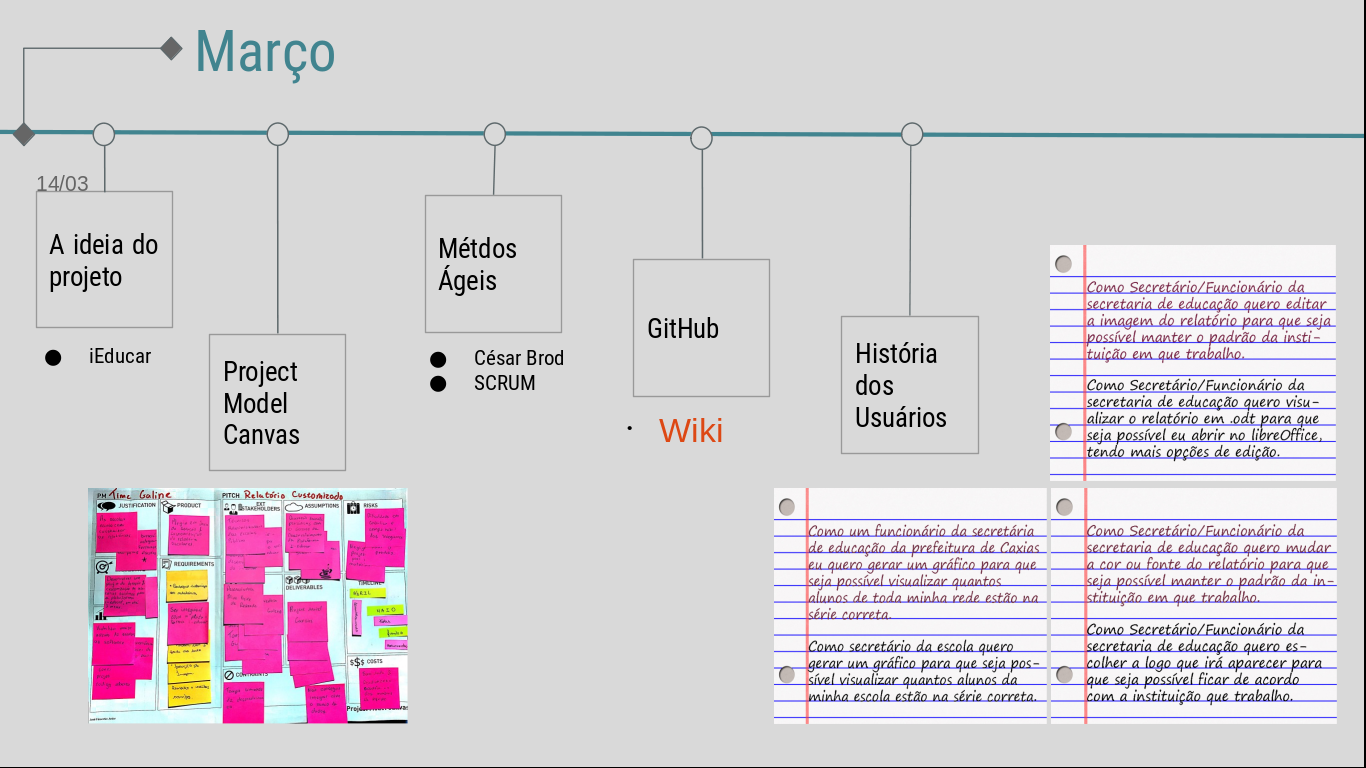
\includegraphics[width=.9\textwidth]{chaps/Images/Linha-tempo1.png}
    \caption{FES-UFRJ - Março-2018.}
    \label{fig:linha-dotempo1}
\end{figure}

\begin{figure}
    \centering
    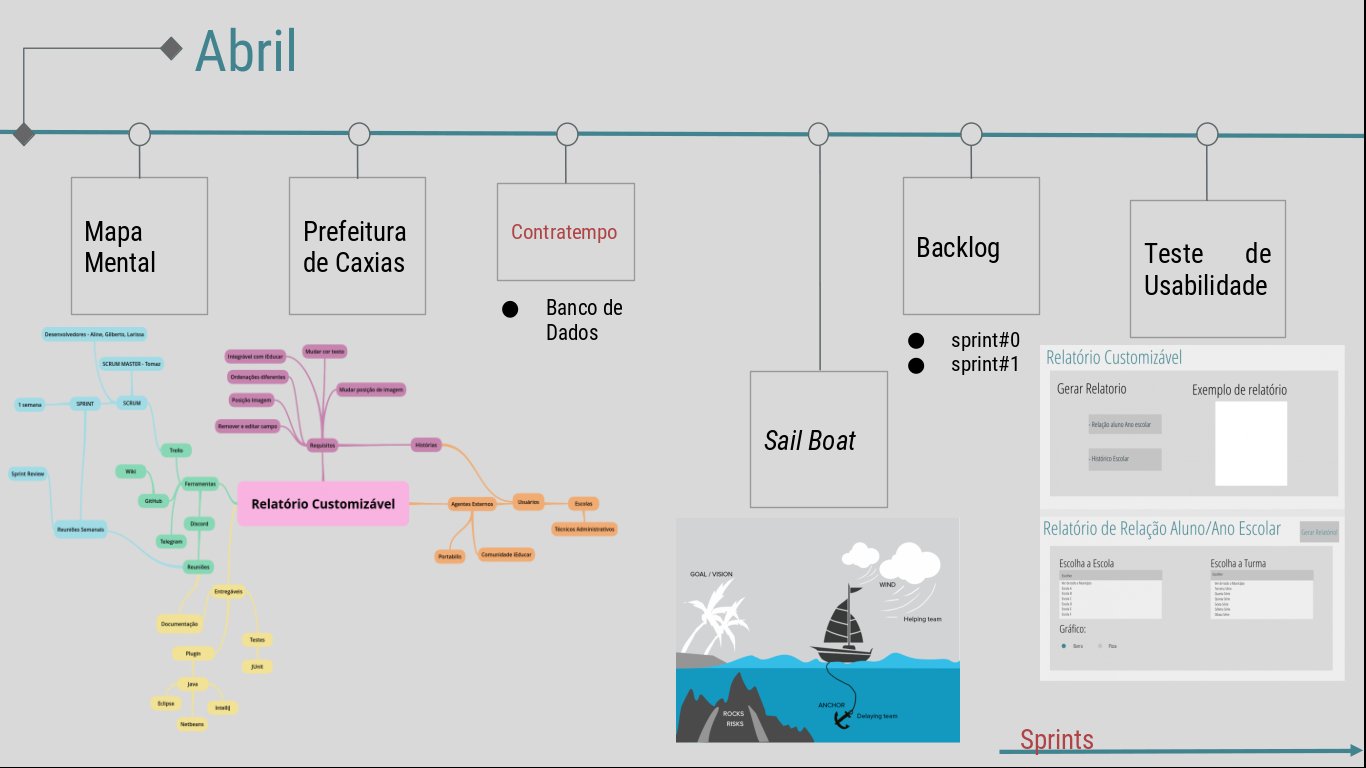
\includegraphics[width=.9\textwidth]{chaps/Images/linha-tempo2.png}
    \caption{FES-UFRJ - Abril-2018.}
    \label{fig:linha-dotempo2}
\end{figure}

\begin{figure}
    \centering
    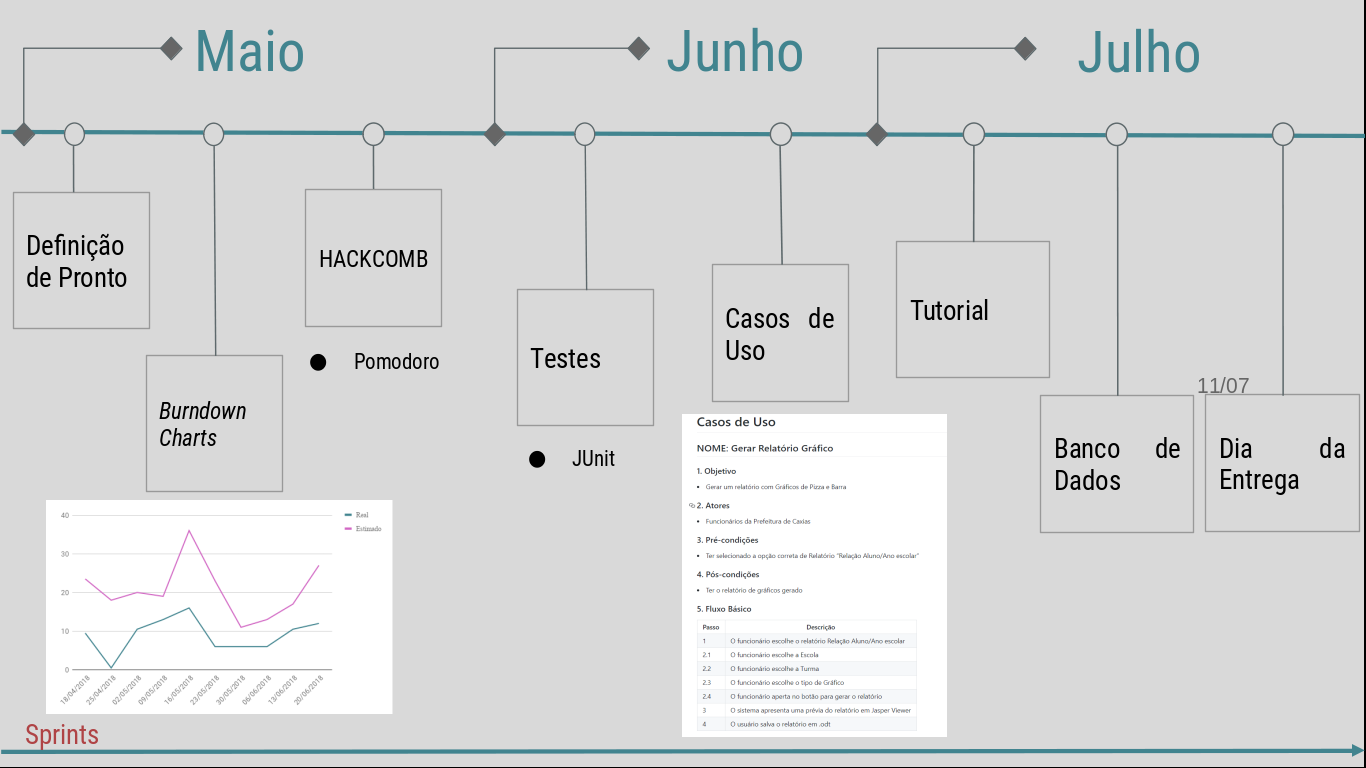
\includegraphics[width=.9\textwidth]{chaps/Images/maio.png}
    \caption{FES-UFRJ - Maio/junho/julho-2018.}
    \label{fig:linha-dotempo3}
\end{figure}


Podemos concluir que os alunos tiveram evolução nas suas habilidades com relação aos temas propostos na aula, conforme uma tabela elaborada por um dos times:

\begin{figure}
    \centering
    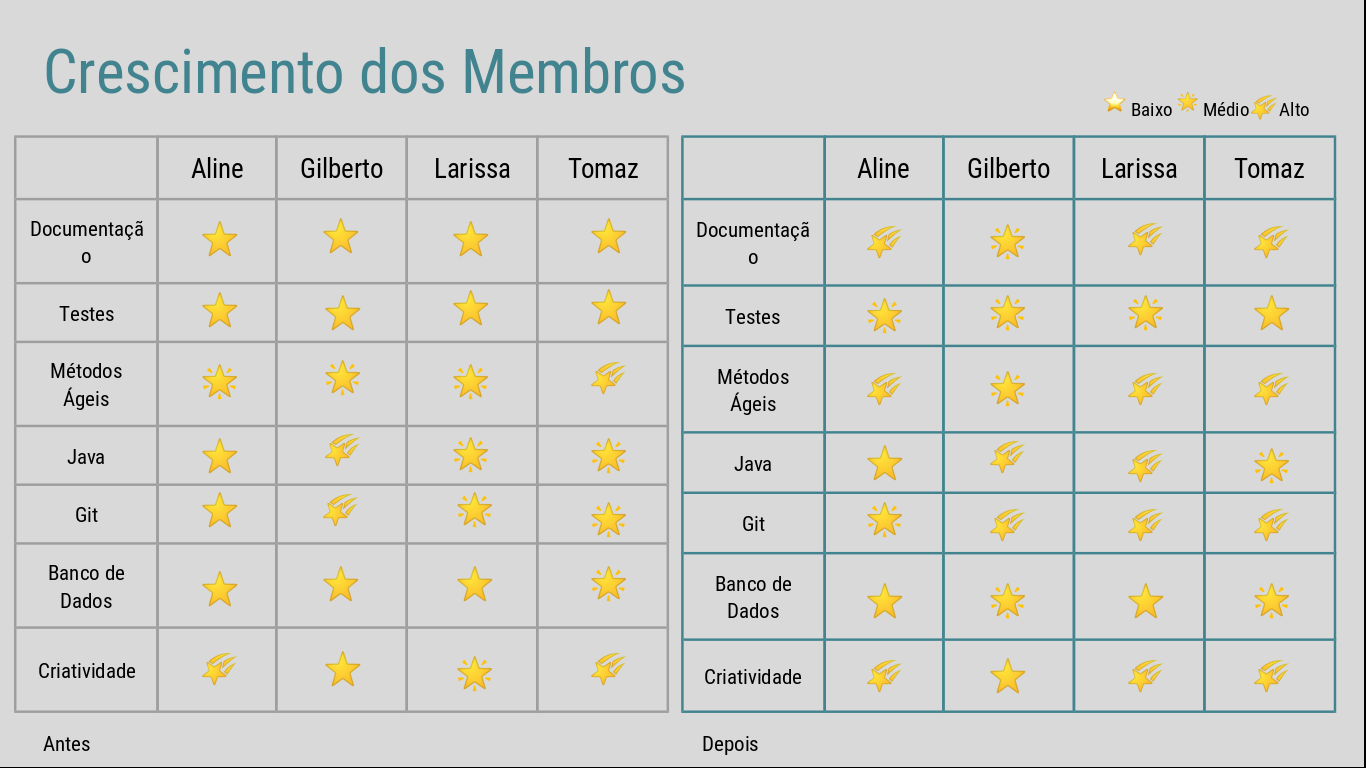
\includegraphics[width=.9\textwidth]{chaps/Images/Habilidades.png}
    \caption{FES-UFRJ - Evolução das habilidades}
    \label{fig:habilidades}
\end{figure}

Todos os times trabalharam com páginas \textit{wiki} de conteúdo aberto que permitiu uma troca de conhecimentos durante as aulas, podendo cada time ver os conteúdos produzidos pelos outros times, também foi disponibilizado um grupo no telegram para continuidade das aulas de forma virtual. Neste grupo existiam a presença de outros especialistas em assuntos diversos, como hackers, desenvolvedores, líderes de comunidades de softwares e especialistas em tecnologia. Todos os alunos compartilhavam suas dúvidas e todos ajudavam. 

Em alguns momentos foram apresentadas tarefas aleatórias com tempo de entrega, onde o primeiro aluno que realizasse a tarefa ganhava uma surpresa, que podia ser um livro, uma camisa ou uma menção honrosa.

Durante as aulas os alunos que conseguiam avançar com alguma atividade, ajudavam os outros que ainda não tinham conseguido realizar. Foram realizadas dinâmicas de meia hora entre os grupos de forma que eles pudessem discutir entre eles algum assunto escolhido para o outro grupo apresentar. Um exemplo disso eram as reuniões virtuais realizadas entre os grupos para ajuda mútua. 

\section{Aplicação do Protocolo Copus}

"Os instrutores e as práticas de ensino que eles empregam desempenham um papel fundamental na melhoria da aprendizagem dos alunos nos cursos de ciências, tecnologia, engenharia e matemática (STEM) da faculdade"(Paper Copus). Em decorrência destas constantes transformações na área da educação, é necessário coletar e analisar informações sobre o que acontece durante o tempo que decorre uma aula. Para que esta análise, principalmente sobre a motivação de estudantes, seja possível, nesta fase da pesquisa usamos um protocolo de observação em sala de aula conhecido como Protocolo de Observação em Sala de Aula para Graduação STEM ou COPUS(Citar). Este protocolo permite que o corpo docente do STEM, após um curto período de treinamento de 1,5 horas, caracterize de forma confiável como o corpo docente e os alunos estão gastando seu tempo na sala de aula(Citar). As aulas monitoradas e preenchidas com a planilha do protocolo(Citar planilha) foram as aulas regulares de Álgebra Linear, ministradas pela Professora Ana Moura Santos na graduação de informática do IST.

Os dados capturados nas observações são referentes a 15 aulas de uma mesma professora e duas outras aulas de dois professores diferentes. As análises que mostraremos abaixo se dividem em três considerando as particularidades da amostra. A primeira análise considera todas as aulas, a segunda somente as aulas da professora com maior frequência, que será nomeada aqui como Professora 1 e a terceira fixa-se somente nos dados das duas aulas dos outros dois professores.

Os dados completos foram analisados à luz de dois algoritmos de classificação baseados em árvore de decisão.
O primeiro algoritmo que foi rodado é o rpart. Por esse algoritmo chegou-se à seguinte árvore simples de decisão mostrada no Gráfico 1.


\begin{figure}
    \centering
    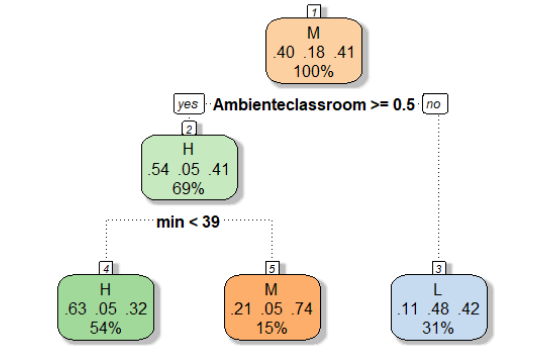
\includegraphics[width=.9\textwidth]{chaps/Images/figura1copus.png}
    \caption{Árvore simples de decisão}
    \label{fig:arvore_simples_decisao}
\end{figure}

A leitura do Gráfico 1 indica que do total das combinações de anotações 41\% são de médio engajamento, 40\% são de alto engajamento e aproximadamente 18\% de baixo engajamento.
Desse total, 31\% dos engajamentos é explicado pelo ambiente de aula ser diferente de sala de aula, ou seja, as aulas acontecem em anfiteatro. Nesses casos, temos que 31\% das combinações referem-se a baixo engajamento.
Para os 69\% restantes há um ponto de decisão referente ao tempo de aula. Até os 39 minutos de aula há uma associação de 54\% das ocorrências para alto engajamento. No caso contrário, há 15\% das associações a médio engajamento.
Temos então que as duas situações mais importantes para o modelo usado, a ponto de aparecerem na árvore de decisão, são o ambiente onde ocorre as aulas e o tempo de aula.
A opção inicial pelo uso da árvore simples deve-se principalmente pelo fato dos seus respectivos modelos serem fáceis de ser interpretados como na figura acima. Para os objetivos desse trabalho que se referem a descrever quais variáveis e quais condições mais influenciam no engajamento dos estudantes, o uso dessa abordagem para uma primeira descoberta é válido. Porém existem outras implementações de uso de árvores de decisão que são mais robustas, principalmente para fazer predições de classificação a partir de dados observados. A desvantagem dessas outras implementações relaciona-se ao fato de não gerarem modelos tão intuitivos. Para este trabalho optou-se por uso de Floresta Aleatória, uma implementação mais robusta de árvores de decisão, para identificar outras variáveis importantes que não tinham sido destacadas quando do uso de árvore simples.
Muito embora o uso de Floresta Aleatória não permita identificar os pontos de gatilho para as decisões, como ocorrem nas árvores simples, foi possível identificar duas novas condições importantes para o modelo. Veja a tabela abaixo.



Pela tabela acima, percebe-se novamente a condição de aula em sala de aula e o tempo de aula, porém agora aparece com destaque mais duas outras condições, uma relacionada a ações dos professores e outra a ação de estudantes, respectivamente FuP e OG.
A importância das quatro variáveis ou condições mais importantes levantadas pelas análises de árvores de decisão podem ficar mais claras através das análises gráficas. As figuras abaixo trazem essa evidência.
O Gráfico 2 mostra a importância do ambiente onde ocorre a aula, especificamente da condição de aula em sala de aula. É possível também perceber a importância do tempo de aula, já que é um gráfico de linha com o tempo representado no eixo horizontal


\begin{figure}
    \centering
    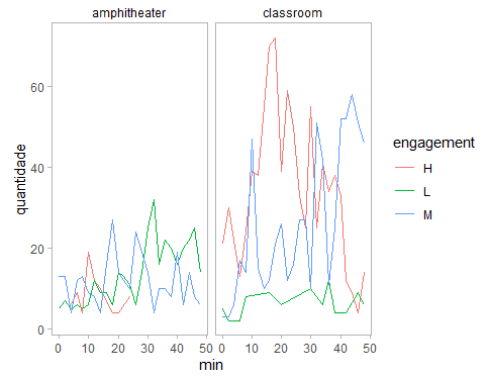
\includegraphics[width=.9\textwidth]{chaps/Images/figura2_copus.png}
    \caption{Árvore simples de decisão}
    \label{fig:arvore_simples_decisao2}
\end{figure}

\section{Aplicação de Escape Room}

Escape Games educacionais são considerados uma estratégia de aprendizado ativo, à medida que os alunos resolvem problemas relacionados com o conteúdo curricular para "escapar" do lugar físico onde eles estão “bloqueados”. Nesta seção é descrita a implementação de dois Escape Games voltados para estudantes de graduação em Ciência da Computação, no Instituto Superior Técnico da Universidade de Lisboa. O procedimento seguido para criar os jogos é apresentado e ambas as atividades são descritas e avaliadas. Além disso, dicas para professores dispostos a construir jogos de fuga educacionais semelhantes são sugerido. Nosso objetivo era entender: a) se os alunos são motivado para este tipo de experiência de aprendizagem; b) se os alunos são ciente dos possíveis ganhos de aprendizagem ao participar nestes Atividades; c) se os alunos, efetivamente, sentem que têm aprendido algo; d) quais são as conquistas desse tipo das atividades (percebidas pelos professores). Considerando o feedback dado pelos alunos: eles se envolvem neste tipo de atividade, estão cientes dos ganhos de aprendizagem e sentem que foi um experiência de aprendizagem frutífera. Além disso, esta atividade foi considerada um sucesso pela corpo docente / equipe organizadora, sendo premiada como uma das boas práticas da universidade.

Embora o ensino tradicional, com base nas aulas tradicionais, tenha sido mostrado ser menos eficaz do que outras alternativas \citep{freeman_active_2014}, no Século 21 continua sendo a principal metodologia de ensino no ensino superior (ES)\citep{wanner_enhancing_2015, yeung_online_2016}. As razões são diversas, nomeadamente que as aulas têm vantagens \citep{webster_defence_nodate}, como transmitir conhecimento em um curto espaço de tempo para um grande número de alunos \citep{gregory_lecture_2013}, garantindo que a transmissão seja correta e precisa. Além disso, muitas vezes falta ao corpo docente a formação pedagógica que facilitam a mudança, como formação pedagógica em ES, ao contrário de outros níveis de ensino, não é obrigatório \citep{jensen_higher_2011}. Na maioria dos países europeus “a maioria dos professores começa a ensinar sem nem cinco minutos de treinamento sobre como fazê-lo ” \citep{rugarcia_future_2000}. Além disso, as políticas universitárias que priorizam publicações / pesquisas sobre o ensino, limitam o tempo e energia disponível para mudar as práticas estabelecidas \citep{waldrop_science_2015}. No entanto, as vantagens dos métodos centrados no aluno, como o aprendizado ativo, estão bem documentadas \citep{prince_does_2004}. Os benefícios da implementação de tais estratégias são o envolvimento dos alunos com o material \citep{ghilay_tbal_2015}, melhor desempenho acadêmico \citep{freeman_active_2014}, "níveis mais elevados de confiança em suas habilidades de resolução de problemas de engenharia" \citep{felder_longitudinal_1997} e menos evasão de alunos \citep{pundak_attitudes_2010}. Dado que “as elevadas taxas de reprovação e evasão dos alunos dos cursos de engenharia têm sido motivo de preocupação para muitas instituições de ensino superior portuguesas” \citep{williams_using_2010}, a aprendizagem ativa representa uma abordagem relevante. Complementarmente, existem recomendações, nomeadamente da Comissão Europeia, para fomentar o desenvolvimento de competências transversais no ES de forma a evitar o “descompasso de competências” (Comissão Europeia, 2012) entre o que a indústria exige dos licenciados e o que os alunos aprendem. Essas habilidades transversais incluem trabalho em equipe, comunicação, criatividade, autorregulação e resiliência. Considerando que os alunos de hoje passam um tempo significativo jogando jogos, a introdução de elementos de jogos na educação - aprendizagem baseada em jogos - é uma tendência crescente em ambientes educacionais, incluindo ES \citep{clarke_escaped_2017}. Os Jogos Educacionais de Escape Room reúnem os benefícios educacionais da aprendizagem ativa, o desenvolvimento de habilidades transversais, a colaboração e a alegria de jogar. Aproveitando a dinâmica do jogo e criando um ambiente de aprendizagem envolvente, no qual os alunos se comunicam e trabalham em equipe para resolver diversos problemas relacionados com os conteúdos, foram implementados dois Escape Games com alunos de Informática (CS), no Instituto Superior Técnico da Universidade de Lisboa. Essas atividades aconteceram nos cursos de Lógica para Programação (LP), nosso estudo piloto, e Álgebra Linear (LA). A partir de agora nos referiremos à primeira experiência como EscapulISTe? -LP e a última como EscapulISTe? -LA. Nossas perguntas de pesquisa foram:

\begin{itemize}
    \item RQ1: Os alunos estão motivados para este tipo de aprendizagem experiência?
    \item RQ2: Os alunos estão cientes dos ganhos de aprendizagem desses Atividades?
    \item RQ3: Os alunos sentem que podem aprender com o Escape Game?
    \item RQ4: Quais são as principais realizações de acordo com o professores?
\end{itemize}

Nesta seção, damos uma descrição detalhada do procedimento que seguimos na criação e implementação Escape Games, com o objetivo de compartilhar o que percebemos como bom práticas e "não fazer" a serem evitados durante a preparação de essas atividades. Assim, esperamos que nossos experimentos possam ajudar outros professores de ES a se concentrarem na importância de se divertindo enquanto prepara uma atividade para envolver seus alunos sobre o assunto. Esta seção está organizada da seguinte forma: Começamos com um contexto teórico explicando porque Escape Games constituem uma estratégia de aprendizagem ativa valiosa em educação STEM (Sub-Seção 2). Na Sub-Seção 3, as duas implementações de Escape Games (EGs) são descritas. Na Sub Seção 4, a avaliação de ambos os jogos é apresentada, e na Sub-Seção 5 nós apresentamos as lições aprendidas durante sua criação e implementação. Encerramos apresentando algumas conclusões e trabalhos futuro (Sub-Seção 6).

\subsection{Bases Teóricas}

A aprendizagem ativa pode ser definida como "qualquer curso relacionado que todos estudantes em uma sessão de aula são chamados a fazer além de simplesmente assistir, ouvir e tomar notas ”\citep{felder_active_2009}. Estratégias de aprendizagem ativa promovem a atividade do aluno e a motivação \citep{prince_does_2004}. Sua implementação em uma classe varia de pausando uma palestra para propor um exercício rápido ou mesmo mudando completamente a dinâmica da classe. Um EEG em que os quebra-cabeças são preparado para fazer os alunos aprenderem algo novo ou praticarem aprendizagens anteriores é uma aprendizagem ativa. Além disso, estudantes  colaboram uns com os outros para resolver os quebra-cabeças. A colaboração pode alavancar a aquisição de outros tipos de conhecimento, como a interação social promovendo a aprendizagem de técnicas e habilidades transversais \citep{tadjer_improving_2020}.

EGs são definidos como jogos baseados em equipes de ação ao vivo (geralmente 5 a 7 pessoas), onde os jogadores descobrem pistas e resolvem quebra-cabeças, “Trancado” em um cômodo ou casa, para cumprir uma meta específica (geralmente escapando), em um período de tempo limitado e normalmente de uma hora \citep{nicholson_peeking_2015}. Eles foram apresentados ao público como atividades recreativas, mas logo a emoção se espalhou para áreas educacionais. Quando aplicado à educação, os EEGs promovem o desenvolvimento de habilidades transversais, como trabalho em equipe e comunicação eficaz porque, em vez de jogar atrás de uma tela, participantes estão colaborando com pessoas reais \citep{nicholson_creating_2018} em tempo real e trabalhando para atingir um objetivo comum. Pensar de forma criativa é crucial neste processo, pois eles encontram diferentes desafios que precisam ser resolvidos de novas maneiras \citep{wiemker_escape_2015}. Resiliência e a autorregulação também são incentivadas, pois diversos estudos relatam que os alunos se sentem frustrados durante a atividade \citep{hermanns_using_2017}.

Embora os autores apresentem isso como uma lacuna, a sensação de frustração é comum, não só ao jogar, mas também em múltiplas situações de vida. Portanto, se devidamente explorado e preparado, participar do EG ajuda o jogador a implementar a auto-regulação, para manter uma postura calma diante dos outros, e continuar trabalhando na solução apesar da frustração. A capacidade de entregar resultados sob pressão é uma habilidade com alta demanda no mundo da engenharia \citep{harun_employability_2017}. Além de ajudar a consolidar conhecimentos e valorizar habilidades transversais, EEG são essencialmente jogos. Alunos nascidos em um mundo de tecnologia massificada, tem acesso a um abundância de plataformas de entretenimento digital que antes gerações não possuiam \citep{osmanovic_beyond_2016} e são parte de uma rede hiperconectada da sociedade digital \citep{buitrago-ropero_digital_2020}. Os EEGs representam uma fonte de motivação devido à semelhança com outros tipos de jogos. Por isso parece correto aplicá-los em um ambiente universitário, dado seu “apelo e valor educacional” \citep{clarke_escaped_2017}.

Houve várias implementações de EEG em ES com resultados promissores. Em um estudo desenvolvido com estudantes de farmacologia \citep{hermanns_using_2017}, 72,2\% dos participantes reconheceram que aprenderam os conceitos abordados durante o jogo e afirmou que a atividade lhes permitiu pensar fora do caixa. Em uma experiência baseada em nutrição saudável \citep{yachin_promoting_2019}, os autores encontraram um aumento após a participação com significância estatística, não apenas no número de respostas corretas a um pós-questionário (em todas as perguntas, exceto uma), mas também na automotivação dos alunos. Dos alunos participando de um eletroímã EG \citep{hou_exploring_2012}, 74\% relataram ter entendido melhor o assunto com o jogo do que com livros didáticos; e em um ambiente de robótica educacional, a maioria dos participantes reconheceram a “usabilidade como ferramenta de ensino” do EG \citep{giang_exploring_2020}. Em um ambiente de química \citep{dietrich_escape_2018}, a maioria dos participantes indicaram que a atividade ajudou a desenvolver a construção da equipe (96\%) e comunicação (90\%).

\subsection{Implementando Escape Games Educacionais}

A preparação complexa envolvida neste tipo de jogos é muitas vezes considerado uma desvantagem potencial \citep{wiemker_escape_2015}, como a maioria dos professores não são especialistas em EG. No projeto atual, duas funções principais dentro a equipe organizadora foi criada - o designer e o professor com experiência no conteúdo (a partir de agora, conteúdo especialista). Essa escolha ajudou a lidar com a complexidade, pois o especialista em conteúdo não está envolvido no design do jogo e o designer não precisa pensar sobre o desafio específico. No entanto, os desafios e seu fluxo, muitas vezes precisam ser repensado pelo designer, de acordo com as instruções do conteúdo de especialistas, pois o especialista é aquele com o conhecimento para decidir o que vai levar à melhor experiência pedagógica. Assim, alguma negociação é necessária entre as partes. A criação e implementação de ambos os EEGs é apresentada no próxima seção.

\begin{figure}
    \centering
    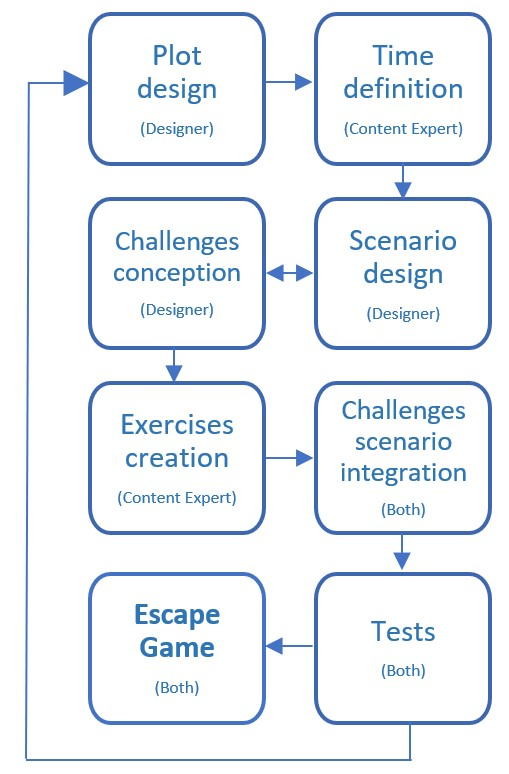
\includegraphics[width=.9\textwidth]{chaps/Images/Esquema Escape(1).jpg}
    \caption{Construindo o Escape Game Educacional.}
    \label{fig:esquema_escape}
\end{figure}

\subsection{Procedimento Geral}

O procedimento seguido pode ser visualizado na Figura 1. Em uma primeira etapa, o designer define o enredo do jogo e o especialista em conteúdo decide quando a experiência deve ocorrer. Uma vez que essas restrições sejam estabelecidas, o designer pode funcionar no cenário - depende da história, mas também do orçamento - e conceituar os desafios. O número de desafios deve ser definido juntamente com o resultado de cada desafio dentro do fluxo do jogo \citep{csikszentmihalyi_creativity_1996}. Por exemplo, o designer pode decidir que a saída do desafio 1 abre um armário com três números e o desafio 2 prompts de saída a senha. Em seguida, o especialista em conteúdo é solicitado a criar N exercícios, um para cada desafio. Por exemplo, considerando o exemplo anterior, o especialista em conteúdo cria exercícios de forma que o o primeiro resultado do exercício corresponde a três números, e o o segundo exercício retorna seis letras e três números (ou seja, um senha).

Em seguida, os desafios são implementados no cenário real, e o jogo está pronto para ser beta testado, preferencialmente por alunos com a mesma formação dos participantes finais. Um desafio frequentemente citado na literatura é que alguns jogadores aprendem as regras do jogo ao invés dos conteúdos educacionais \citep{sanchez_teaching_2019}, criando uma experiência superficial \citep{nicholson_creating_2018}. Este aspecto pode ser minimizado com uma definição prévia de resultados de aprendizagem rigorosos e objetivos \citep{waldrop_science_2015}, mas também com um debriefing cuidadoso no final da atividade para garantir a reflexão e metacognição \citep{sanchez_teaching_2019}. Isso pode ser feito durante os testes beta, o que pode levar a alterações em todo o conjunto de etapas anteriores. Obter feedback de testadores e participantes e refletir sobre a experiência pode ajudar o designer e o especialista em conteúdo realizarem rearranjos e correções. Além disso, após as implementações iniciais, os professores podem construir mais confiança para ampliar a experiência \citep{borrego_room_2017}. Ainda nesta etapa de validação, e antes de apresentar o jogo final aos alunos, uma última ação deve ser realizada: uma diretriz detalhada deve ser fornecida e testada pela equipe organizadora, ou um membro da equipe, que será responsável por preparar a sala após cada implementação.

Todo o rearranjo de ações necessário deve ser detalhado com precisão em uma lista ordenada, que deve ser rigorosamente seguida. Só então o EEG está pronto para ser executado (passo 6). Porém, ainda existem alguns procedimentos a serem seguidos. Em cada sessão, um dos organizadores da equipe se reúne com a equipe de cada aluno e explica o enredo. Nesse momento, os alunos são convidados a assinar um formulário declarando que não vão discutir a atividade com outros alunos e que cuidarão bem dos materiais. Após cada implementação do jogo, ou o professor se reúne com a equipe dos alunos para um breve debriefing, ou uma pesquisa pode ser aplicada a fim de garantir que os alunos refletem sobre a atividade e reconhecem possíveis aquisições de outras habilidades. Depois que todas as equipes participarem, é proposto um questionário a todos os alunos, a fim de avaliar a atividade.

\subsection{Plot Design e Definição do tempo}

Uma narrativa que ajuda a “Definir a atmosfera do jogo e estabelecer as bases do investimento emocional e da curiosidade junto com o jogador" \citep{clarke_escaped_2017} é uma peça importante no projeto de EEG. No nosso caso, um personagem foi criado: Anita, uma estudante de Ciência da Computação que adora EG. Em EscapulISTe? -LP, estudantes se reuniram no quarto de Anita para estudar Lógica. Eventualmente, eles adormecem. Então acordam para descobrir que Anita os trancou e deixou vários desafios de LP que eles precisam resolver para escapar da sala. Eles têm uma hora para fazer isso, ou será tarde demais para o exame. O EscapulISTe? -LP foi implementado no final do semestre e antes do primeiro exame. Portanto, os alunos podem relembrar os principais tópicos antes de se preparar para o exame e testar seus conhecimentos prévios.

Em relação ao EscapulISTe? -LA, Anita fica trancada dentro do armário enquanto prepara um EEG sobre LA. Ela manda um e-mail pedindo ajuda. Os estudantes devem resolver os desafios para abrir o armário e ter uma hora para fazê-lo, ou ela não conseguirá respirar e morrer. EscapulISTe? -LA foi planejado para ser implementado antes do teste intermediário. Essa escolha se baseou em dois motivos. Em primeiro lugar, os desafios estavam relacionados aos conceitos algébricos que possuem saídas numéricas. O segundo motivo para esse planejamento foi pedagógico - no momento do teste de meio de semestre, os alunos geralmente estão sobrecarregados com os projetos de outros cursos e têm um desempenho pior, em comparação com o primeiro teste.

\subsection{Scenario design}

Todos os elementos do EEG devem ser integrados em um conjunto coerente que promova uma experiência envolvente e significativa. O espaço físico e a narrativa devem ser combinados, com a ajuda de decorações e objetos \citep{guigon_model_2018}, para criar um enredo plausível. Nosso primeiro desafio foi criar uma sala de Anita confiável. Isso foi possível com a doação de diversos móveis. Além disso, definimos traços em relação à “personalidade” de Anita: ela adora a seleção nacional de futebol, livros e Harry Potter. Detalhes da decoração como uma foto da seleção nacional e uma camiseta de Harry Potter foram introduzidos. O cenário para LP pode ser visto na Figura 2.

\begin{figure}
    \centering
    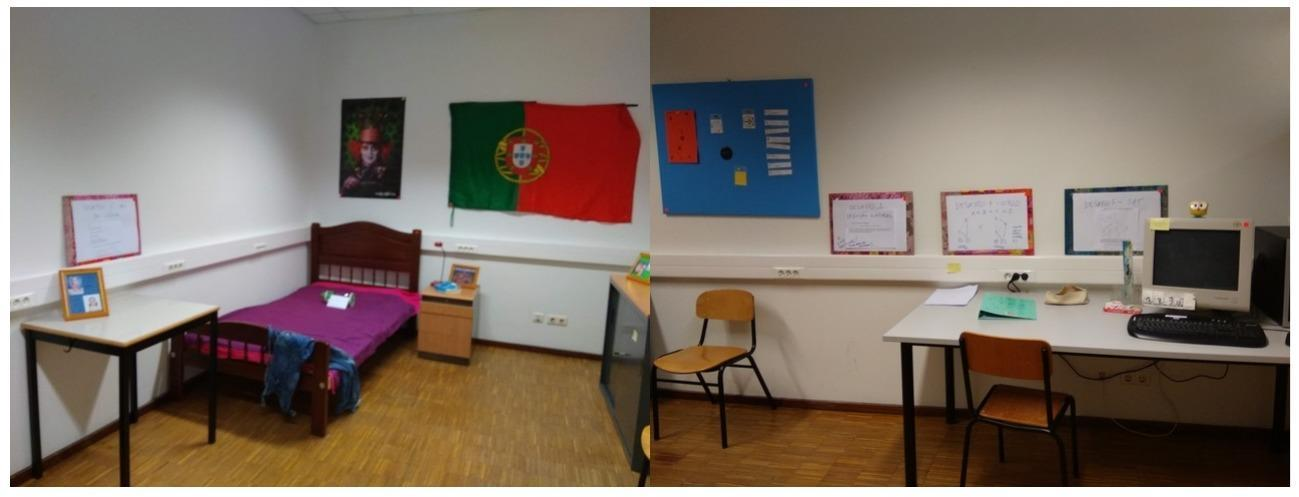
\includegraphics[width=.9\textwidth]{chaps/Images/Figura2(1).jpeg}
    \caption{Quarto da Anita}
    \label{fig:quarto_anita}
\end{figure}

\subsection{Challenges conception}

Ao contrário do que se pode constatar no EG ao vivo e dados os objetivos pedagógicos, é contraproducente o aluno perder tempo com pistas falsas. Assim, em ambas as implementações, os alunos tiveram cinco exercícios para resolver, explicitamente numerados. Posteriormente, foi definido o fluxo dos cinco desafios, determinando, por exemplo, que o primeiro abrisse o armário X que permitiria aos alunos o acesso ao segundo desafio, com uma ordem estrita de ações. As fechaduras estavam presas a um carrinho, uma mochila, uma maleta e duas caixas. Alguns deram chaves para abrir a gaveta da mesinha de cabeceira ou do guarda-roupa, onde os alunos encontravam os exercícios escritos.

A integração do EEG em áreas não numéricas pode representar um desafio adicional, pois as soluções para abrir as fechaduras são geralmente numéricas \citep{guigon_model_2018}. Em nossa experiência, mesmo em cursos STEM, às vezes o tipo de exercícios não se ajusta precisamente a uma meta numérica. Sempre é possível, em qualquer conteúdo, adotar uma abordagem criativa onde as palavras se transformam em números e explorar outras maneiras de desbloquear fechaduras.

\subsection{Exercises creation}

Após a definição do número de desafios e seu fluxo, os especialistas em conteúdo criaram os exercícios para seu tópico de especialização, considerando as orientações fornecidas pelo designer. A concepção dos exercícios baseou-se nos objetivos de aprendizagem traçados para o EEG. Para álgebra linear (EscapulISTe? -LA), por exemplo, cinco objetivos de aprendizagem foram estabelecidos:

\begin{itemize}
    \item Manipulando equações da matriz
    \item Inversos de matriz de computação
    \item Aplicação de propriedades de matrizes de Markov
    \item Determinantes de computação
    \item Manipulação de matrizes particionadas
\end{itemize}

Em seguida, foram preparados diferentes exercícios de álgebra de matrizes, matrizes inversas, matrizes de bloco e determinantes. Aqui estão dois exemplos de exercícios específicos:

\begin{itemize}
    \item Considere a matriz simétrica [fornecida explicitamente]. Você precisará descobrir as entradas da terceira coluna da matriz inversa.
    \item Considere a matriz de Markov [fornecida explicitamente com três entradas ausentes] com o vetor estacionário .... (OOPS, você precisa descobrir!). A chave que você precisa encontrar é composta pelas entradas ausentes na matriz.
\end{itemize}

Para EscapulISTe? -LP, os exercícios propostos progrediram da dedução natural e representação lógica de primeira ordem para diagramas de decisão binários ordenados. Além disso, um programa em Prolog (com um bug) foi fornecido. Quando o bug foi corrigido, um número foi retornado e os alunos puderam acessar o próximo desafio.

\subsection{Challenges scenario integration}

Inúmeras ideias de desafios podem ser implementadas. Aqui são três exemplos usados no projeto atual:

\begin{itemize}
    \item Um dos números abre uma caixa com um ímã dentro. Este ímã permite que os alunos removam uma chave no fundo de uma caixa transparente longa e estreita.
    \item Aproveitando o fato de que a lógica estava sendo ensinada, os alunos precisaram decifrar três fórmulas na lógica de primeira ordem para encontrar a ordem de três xícaras numeradas.
    \item Tinta invisível foi usada para escrever informações importantes sob a cama de Anita. Durante o jogo, os alunos encontraram uma lanterna de luz negra e uma pista do livro de Calvin e Hobbes, "Monstros debaixo da cama".
\end{itemize}

\subsection{Beta tests}

Antes da implementação final com os alunos, professores voluntários testaram ambos os jogos. Muitas pistas foram repensadas na época. Para EscapulISTe? -LP, nosso estudo piloto, cinco alunos de CS também foram convidados a jogar o jogo. Com o feedback deles, conseguimos entender quais desafios eram muito complicados ou muito fáceis. Para o EscapulISTe? -LA, vários alunos de diferentes anos e graus se ofereceram para testá-lo. Um debriefing ocorreu após cada sessão experimental e o feedback geral permitiu uma reflexão sobre a experiência e promoveu várias correções. Em relação às orientações para reorganizar a sala, o designer do jogo forneceu uma lista detalhada com os códigos do armário e as 25 etapas necessárias para ter todos os objetos na posição correta. Esta foi uma peça fundamental e professores / equipe organizadora responsáveis pelas implementações praticaram a tarefa de antemão, várias vezes. Se algo falhasse, a próxima implementação seria comprometida.

\subsection{Avaliação}

O EscapulISTe? -LA foi proposto aos 90 alunos matriculados no primeiro ano de Ciência da Computação, em novembro de 2019, antes do exame de meio de semestre. Embora a atividade fosse opcional, teria um impacto irrisório na nota final (cerca de 1,5\%). Aconteceu durante oito dias da semana, duas equipes por dia. Os alunos foram organizados em equipes (5 alunos cada), inscrevendo-se previamente num sistema de matrícula desenvolvido por um aluno bolseiro. Este registro online facilitou a organização das equipes de alunos por vagas disponíveis e nos permitiu manter um registro da participação dos alunos. Dos 90 alunos, 79 alunos se inscreveram para a atividade. Desta vez não houve “spoilers” e cada grupo demorou entre 40 a 55 minutos para resolver os desafios. Novamente, após cada sessão, um breve debriefing foi feito. Quando todas as equipes terminaram a atividade, um questionário foi realizado através do nosso Sistema de Gestão de Aprendizagem (LMS). Dos 90 alunos, foram coletadas 66 respostas (8 mulheres e 58 homens), 63 respostas de alunos que participaram do EscapulISTe? -LA e 3 de alunos que não participaram. Além disso, em conversas informais com os organizadores, eles puderam compartilhar sua experiência sobre se sentirem às vezes frustrados durante a atividade, mas felizes por terem superado isso com a ajuda do grupo.



\subsection{EscapulISTe? -LP Feedback dos alunos}

EscapulISTe? -LP foi o piloto e o objetivo principal foi obter insights a partir da experiência. Sete equipes (3-6 alunos) participaram (um total de 33 alunos do primeiro ano de CS), até o final do semestre da primavera. Se algum dos desafios for muito complicado, eles adicionam acesso a “spoilers”, já que as soluções dos desafios foram escritas no verso de quadros coloridos (Figura 2). Após cada sessão, um breve debriefing foi feito. Alguns dos grupos marcaram um ou dois “spoilers”, mas a maioria dos alunos conseguiu “escapar” sem ajuda, geralmente em cerca de 45 minutos.

Os alunos foram convidados a dar feedback informal, com a possibilidade de anonimato. Temos 24 respostas, e apenas comentários positivos como: “foi muito bom! [...] reveja o materiais [...] realmente criativos ”,“ Foi uma experiência legal. [...]
muitos tópicos foram revisados [...] formas alternativas de estudar,
mais divertida e também diferente ”,“ Legal !!!! ”.

\subsection{Avaliação do EscapulISTe? -LA}



\section{Mapeamento Sistemático de Autorregulação da Aprendizagem}

\section{Análise de dados no MOOC Técnico}

Neste relatório faz-se a análise de dados de três edições consecutivas dos cursos online “Controlo e Simulação de Drones” (droneX) e “Transformação Digital” (tdX), disponibilizados na Plataforma MOOC Técnico 1 . No primeiro caso, droneX, referimonos às edições de 2018, 2019 e 2020 e no segundo , tdX, considerámos as edições de 2017, 2018 e 2020. O nosso objetivo é analisar o comportamento de adesão dos 2
estudantes do Técnico Lisboa e de participantes externos inscritos nestes MOOC às atividades de avaliação, identificando padrões no seu desempenho, em particular com base no género, fazendo uma análise conhecida como Learning Analytics, Analytics e acrescentar alguns comentários individuais desses participantes enquanto avaliadores das atividades e conteúdos do droneX e do tdX. A análise com base no gênero é importante 3 no contexto da participação do MOOC Técnico no projeto
europeu FOSTWOM (2019). Este projeto tem como objetivo principal atuar na falta de equilíbrio de género nas áreas STEM, usando o potencial democrático dos MOOC.

Para a análise de dados usamos as pautas das avaliações para cada uma das edições
MOOC (em formato .csv) e fichas de perfil dos inscritos (em formato .csv), ambas
geradas pela plataforma e retiradas no final de cada edição. Incluímos ainda dados de
questionários iniciais e questionários finais. Estes últimos são respondidos via Google
Forms, mas acedidos diretamente na plataforma em cada uma das edições droneX e tdX. Como contextualização indicamos os objetivos gerais, o público alvo e a organização das atividades de avaliação, em cada um dos casos, droneX e tdX. Pontualmente, foram analisados os arquivos das pautas finais do Fénix  da UC  de “Controlo de Voo” para comparação de números de estudantes inscritos nesta UC com números totais de inscrições no MOOC droneX.

Para a análise,
escolhemos os seguintes para tratar os seguintes indicadores: taxa de Completion Rate
sucesso (Completion Rate) no MOOC em cada uma das edições sucessivas dos dois cursos online; distribuição de participantes por género em cada uma das edições; número de participantes inscritos com filiação IST; taxa de sucesso relativo por género, ou seja, participantes femininos/masculinos com sucesso entre participantes inscritos femininos/masculinos; comentários de satisfação dos participantes quanto às atividades avaliativas e quanto às expectativas iniciais sobre o MOOC (dados
qualitativos).

Na realização das análises mais estruturadas usámos RStudio, que é um software
livre de ambiente de desenvolvimento integrado para linguagem R. A linguagem R é uma linguagem de programação que permite gerar gráficos com base em cálculos estatísticos, permitindo-nos analisar dados agregados provenientes de ficheiros diferentes. É importante destacar que os números apresentados neste relatório provêm de ficheiros (.csv) diferentes, provenientes da plataforma MOOC Técnico, que foram posteriormente agregados para serem tratados no RStudio. Foram agregados em cada caso, droneX e tdX, três ficheiros tipo grade e três ficheiros tipo profile, descarregados a partir da plataforma em datas imediatamente posteriores ao final de cada edição. Numa primeira etapa, os dados agregados foram limpos, uma vez que
enrollees com registos no ficheiro grade que não existem participantes inscritos (enrollees)
estão no ficheiro profile, profile e vice-versa. A agregação feita no RStudio dos seis ficheiros de cada curso online foi feita com base nos indicadores “id”, “username”,
“email”,“ano”(by=c('id','username','email','ano')) através do comando join . Assim, o RStudio
gera relatórios finais com números totais por curso online e por ano, por género, por
Completion rates) rates global ou parcial, por exemplo, usando os dados taxas de sucesso (Completion primários que se comportam bem para os indicadores referidos. Os números gerados
pelo RStudio, e que apresentamos neste relatório, são números que se referem a
estes últimos dados primários.

\subsection{Contexto do MOOC Simulação e Controlo de Drones (droneX)}

O MOOC “Simulação e Controlo de Drones” (droneX) é aconselhado aos estudantes
inscritos na UC “Controlo de Voo” e usado durante os semestres de execução desta
UC numa estratégia de flipped-classroom
flipped-classroom. Em particular, o resultado das atividades de avaliações do MOOC contaram em cada uma das suas edições com uma
percentagem para a nota final da UC, que é uma disciplina do 3o ano do Mestrado Integrado de Engenharia Aeroespacial. Como se pode ler na página About o curso online droneX tem como objetivo analisar o funcionamento de drones multirotores e das partes que os constituem,
saber como desenvolver um simulador para analisar o seu comportamento e projetar soluções para o seu controlo automático.
As atividades de avaliação do MOOC droneX nas suas últimas três edições consistiram em um teste de avaliação de conhecimentos relativo a cada um dos quatro módulos, e um exame final, com questões de escolha múltipla e exercícios
vários, em que cada avaliação contou com 20\% para a nota final. Quando um participante atinge pelo menos 60\% de sucesso nas atividades avaliativas do curso, recebe um Honor Certificate correspondendo a um certificado de participação no curso com sucesso (sem classificação atribuída). É com base no número de certificados emitidos que se calcula a taxa de sucesso no MOOC.


\subsection{Análise dos dados de três edições}

Estiveram inscritos na edição do droneX de 2018 um total de 1258 participantes, entre os quais 424 inscreveram-se mediante autenticação Fénix com IST ID. Nesta edição, inscreveram-se 160 participantes do género feminino, dos quais 50 participantes tiveram sucesso (pelo menos 60\% de sucesso) nas atividades de avaliação do MOOC. Com relação ao género masculino, o total de participantes inscritos foi de 1088, 14 dos quais 312 participantes tiveram sucesso. O número total de participantes femininos e masculinos que terminaram com sucesso em 2018 foi de 362, o Completion rate que resulta numa taxa de sucesso (Completionrate) geral de 29\%.

Em 2019, estiveram inscritos no droneX um
total de 428 participantes, entre os quais 341
inscreveram-se com a autenticação Fénix. Deste número, 69 participantes eram do género feminino, tendo 28 participantes terminado com sucesso. Com relação ao género masculino, o total de participantes foi de 357, tendo 150 participantes terminado com sucesso. O total de participantes femininos e masculinos que tiveram sucesso foi de 178 de participantes femininos e masculinos que tiveram sucesso foi de 178, o que resulta numa Completion rate
taxa de sucesso (Completionrate) total 42\%.

Em 2020, estiveram inscritos 518 participantes,
entre os quais 458 inscreveram-se com a
autenticação Fénix. Nesta edição do droneX,
inscreveram-se 91 participantes do género
feminino das quais 53 foram as participantes
femininas que tiveram sucesso. Com relação ao
género masculino, o total de participantes foi de 420, dos quais 213 tiveram sucesso. O número de participantes femininos e masculinos que
terminaram com sucesso foi de 266, resultando
Completion rate numa taxa de sucesso (Completion rate) geral de 51\%, a mais elevada até ao momento.

\begin{figure}
    \centering
    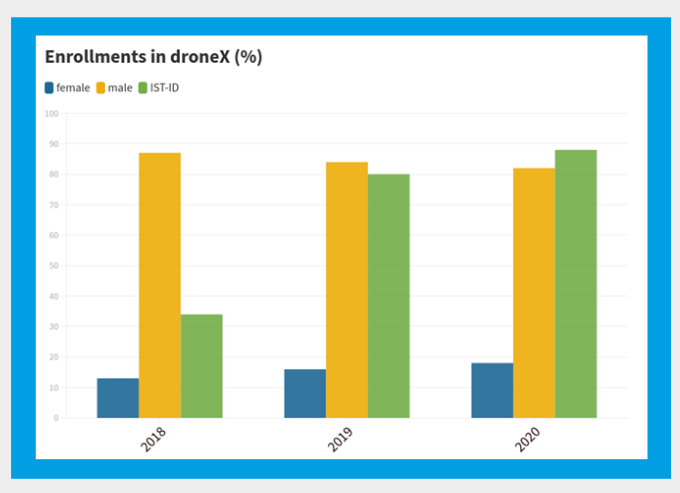
\includegraphics[width=.9\textwidth]{chaps/Images/taxa_insc_dronex.png}
    \caption{Taxas de inscrição nas várias edições do droneX}
    \label{fig:taxa_insc_dronex}
\end{figure}

Na Figura 1, podemos ver a distribuição
em cada ano da taxa de inscrição no
droneX por género (female, male) e a female, male percentagem de inscritos com filiação
IST (IST-ID), que neste caso pode indicar também estudantes inscritos na UC “Controlo de Voo” (ver ainda Fig. 5), ou alumni.

\begin{figure}
    \centering
    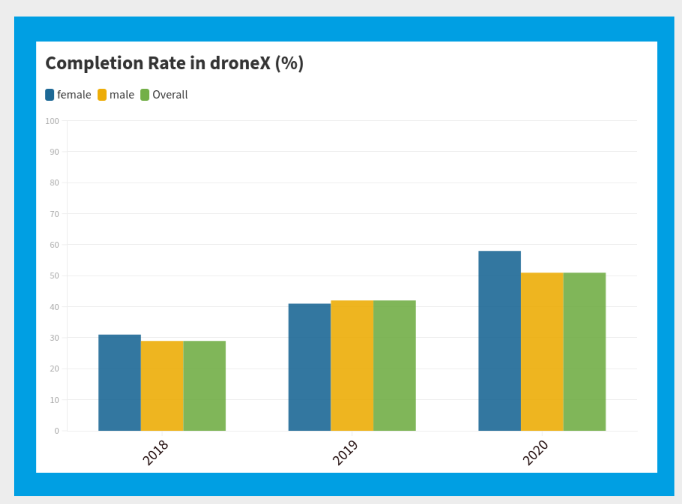
\includegraphics[width=.9\textwidth]{chaps/Images/taxa_sucesso_dronex.png}
    \caption{Taxas de sucesso nas várias edições do droneX.}
    \label{fig:taxa_sucesso_dronex}
\end{figure}

Na Figura 2, podemos ver as taxas de
sucesso (Completion rates) em cada Completion rates edição anual do droneX, percentagens
female, male género (female, female, por female, male male) e a overall percentagem total Overall A partir dos dados referidos
(Overall). acima e da visualização das duas
figuras, podemos concluir que a maioria dos inscritos no droneX são estudantes IST ou alumni do género masculino, e veremos na secção Flipped classroom com UC do Técnico  que só alguns deles são também estudantes inscritos na UC “Controlo
de Voo”.

As taxas de sucesso no droneX, exceto a total e a do género masculino na edição de 2018, situam-se acima dos 30\%. As taxas de sucesso femininas (relativas às inscrições femininas) em 2018 e 2020 ultrapassam as taxas globais.

\begin{figure}
    \centering
    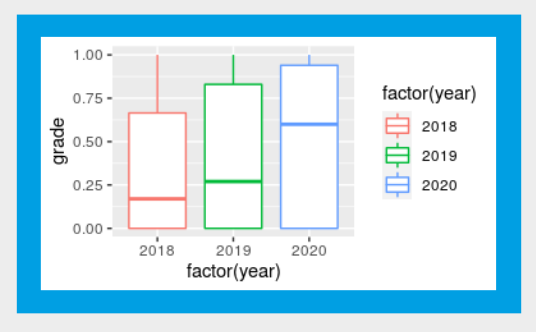
\includegraphics[width=.9\textwidth]{chaps/Images/boxplot_grade_dronex.png}
    \caption{Boxplot para a variável grade por fator year. Para cada caixa temos uma base que representa o primeiro quartil, um traço dentro da caixa que representa a mediana e o segundo quartil simultaneamente, e o topo da caixa que
representa o terceiro quartil.}
    \label{fig:boxplot_grade_dronex}
\end{figure}

No diagrama boxplot da Figura 3 podemos ver a relação entre as notas (numa escala de 0\% a 100\%) dos participantes no curso online droneX ao longo de três anos (2018, 2019 e 2020), com os dados agrupados de grade em relação ao fator year year. Verifica-se uma assimetria positiva para os dados de 2018 e 2019 e uma
assimetria negativa para os dados de 2020. É
importante notar que a mediana (segundo quartil) e o terceiro quartil das notas obtidas no MOOC tem vindo a aumentar ao longo destes três anos, estando em 2020 a
mediana próxima de 60\% e o terceiro quartil próximo dos 94\%. Recordamos que esta última edição decorreu durante um semestre académico marcado pela pandemia Covid-19, em que as aulas e a avaliação passaram para um regime remoto. O interesse e relevância de conteúdos online, em particular os MOOC, aumentaram substancialmente entre o público universitário. A caixa correspondente a 2020 é disso testemunho.

\begin{figure}
    \centering
    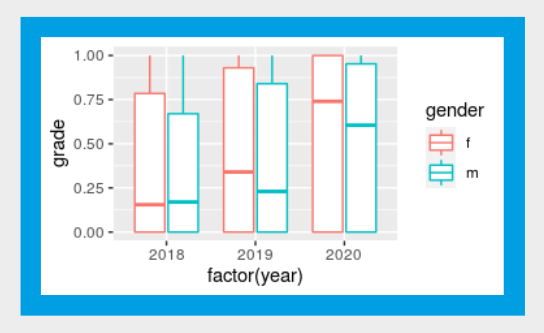
\includegraphics[width=.9\textwidth]{chaps/Images/boxplot_gender_drone.png}
    \caption{Boxplot para as variáveis grade e gender por fator year.}
    \label{fig:boxplot_gender_dronex}
\end{figure}

No diagrama boxplot da Figura 4, podemos ver a
relação entre as notas (numa escala de 0\% a
100\%) dos participantes no curso online droneX agrupados por grade e gender (f=feminino e m=masculino) em relação ao fator year (anos 2018, 2019 e 2020). Verifica-se que as assimetrias por género seguem o mesmo padrão dos dados globais, sendo positivas para os ambos os géneros em 2018 e 2019, e negativas para ambos os géneros em 2020. É importante notar que a mediana (segundo quartil) e o terceiro quartil das notas obtidas pelos participantes do droneX têm vindo a aumentar ao longo destes três anos.

Em geral, as medianas e os valores do terceiro quartil das notas de participantes femininas em 2019 e 2020 são mais elevadas do que as dos participantes masculinos. Por exemplo, em 2020 a mediana feminina encontra-se nos 74\%,
enquanto a mediana masculina está próxima de 61\%, e o terceiro quartil feminino próximo dos 100\%, enquanto o terceiro quartil masculino se encontra próximo dos 97\%. A edição de 2020 foi aquela em que houve mais participantes inscritos com sucesso nas atividades de avaliação, em particular houve muitas notas de participantes femininas próximas dos 100\%.

\subsection{Flipped classroom com
UC do Técnico Lisboa}

Para uma breve comparação entre os dados de inscrições e taxa de sucesso do droneX e da disciplina “Controlo de Voo” fornecem-se os
números abaixo. Dos participantes inscritos nas três edições referidas do MOOC droneX, um
número de 141 participantes em 2018, de 120 em 2019 e de 139 em 2020, eram também estudantes inscritos na UC “Controlo de Voo”.

De entre os 141 estudantes da UC “Controlo de Voo” de 2018, 23 estudantes eram do género feminino, dos quais 4 participantes terminaram com sucesso o droneX. Com relação ao género masculino, 119 estudantes participaram, sendo 7 os que finalizaram com sucesso.

Em 2019, o número total de estudantes inscritos na UC foi de 120. Destes, 23 estudantes eram do género feminino, e 20 destas participantes tiveram sucesso
no droneX. Com relação ao género masculino, 97
estudantes participaram, sendo 72 os que
obtiveram sucesso.

\begin{figure}
    \centering
    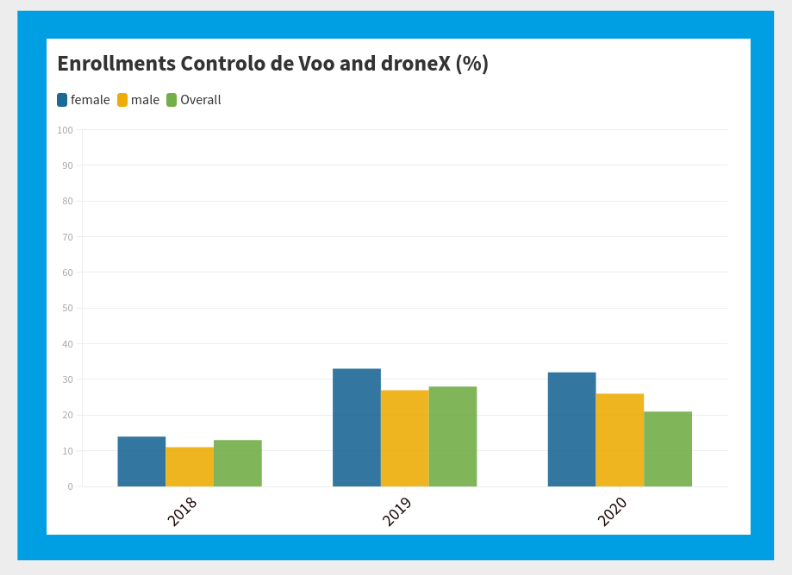
\includegraphics[width=.9\textwidth]{chaps/Images/enrollments_voo_drone.png}
    \caption{Percentagens de inscrição de estudantes da UC no droneX.}
    \label{fig:enrollment_voo_dronex}
\end{figure}

Em 2020, o número total de estudantes inscritos em “Controlo de Voo” foi de 139, dos quais 29 estudantes eram do género feminino. Destas, 27 estudantes ao participarem no droneX, obtiveram sucesso contribuindo para a
mediana próxima dos 75\% referida acima (ver
Fig. 4). Com relação aos inscritos masculinos na UC, 110 participaram no droneX, com 82 entre eles que obtiveram sucesso nas atividades de avaliação.

\subsection{Conclusão sobre a experiência global do MOOC droneX}

Podemos assim concluir que os participantes inscritos nas várias edições do droneX são estudantes IST ou 19 alumni de género masculino, mas só alguns deles são também estudantes inscritos na UC “Controlo de Voo”
(ver Fig. 5).

Relativamente à prestação feminina das várias edições do droneX, queremos sublinhar que embora exista uma percentagem baixa de alunas inscritas na UC de "Controlo de Voo” (entre 16\% e 21\%), e também de participantes femininas no MOOC (ver Fig. 1), estas
últimas alcançaram boas taxas de sucesso no droneX (ver Fig. 4). Recordamos que um dos objetivos principais do projeto europeu FOSTWOM é chamar a atenção para a falta de equilíbrio de género em muitas áreas STEM e
usar a acessibilidade dos MOOC para aumentar a
participação feminina nas áreas de Engenharia.

De modo geral, os participantes demonstraram
estar satisfeitos com as atividades de avaliação e os conhecimentos adquiridos.

Deste modo, quando se desenha e produz um MOOC a pensar em usá-lo como complemento, ou mesmo em aplicá-lo em flipped-classroom a uma UC específica do Técnico Lisboa, está a servir-se uma comunidade académica da escola mais alargada, como estudantes de outras UC e/ou alumni.

\subsection{ANÁLISE DO CURSO ONLINE TRANSFORMAÇÃO DIGITAL}

\subsection{Contexto do MOOC Transformação Digital}

O MOOC “Transformação Digital” (tdX), como se pode ler na descrição da About é aconselhado a todos os profissionais, alunos finalistas
sua página About, (prestes a entrar no mercado de trabalho) e ainda a potenciais empreendedores que tenham interesse em perceber o papel das novas tecnologias nas
organizações, tanto públicas como privadas Os participantes neste curso deverão ter interesse pelas novas tecnologias assim como vontade de transformar as organizações onde trabalham atualmente e/ou criar novos negócios.

Dentro do contexto MOOC Técnico, este MOOC é um curso online transversal para um público alargado, não obrigatoriamente académico, que tem como propósitos tirar partido das novas tecnologias para transformar as organizações, tendo como objetivo final aumentar as vendas, reduzir custos, ou criar novos negócios.

As atividades de avaliação do MOOC tdX nas suas últimas três edições consistiram em 4 exercícios de Peer Review Review. Estes exercícios são enunciados no final de cada tópico. Os participantes devem responder individualmente, sendo as respostas submetidas posteriormente avaliadas pelos seus pares, pequeno grupo de constituição aleatória de outros participantes inscritos. Finalmente, há uma revisão e confirmação da classificação mediana do grupo feitas pelo tutor.
Quando um participante atinge pelo menos 60\% de sucesso nas atividades avaliativas de Peer Review Review, recebe um Honor Certificate
Certificate, certificado de participação com sucesso (sem classificação atribuída). Recordamos que é com base no número de certificados emitidos que se calcula a taxa de sucesso no MOOC.

\subsection{Análise dos dados de três edições}

Em 2017, estiveram inscritos no tdX um total
de 1111 participantes, em que 78\% dos
participantes eram externos ao Técnico Lisboa.
Do total de participantes, 317 corresponderam a inscrições de género feminino, sendo 61 as
participantes femininas que obtiveram sucesso
(pelo menos 60\% de sucesso) nas atividades
de avaliação. Com relação ao género masculino,
21 o total de inscritos masculinos foi de 785, dos quais 162 inscritos obtiveram sucesso. O
número total de participantes que obtiveram
sucesso foi de 223, o que resulta numa taxa de
Completion Rate) geral de 20\%.

Estiveram inscritos na edição do tdX de 2018 um total de 1046 participantes, em que 73\% dos
participantes eram externos ao Técnico Lisboa.
Entre os inscritos, 336 participantes eram do
género feminino, sendo 50 as participantes que
obtiveram sucesso. O total de participantes de
género masculino foi de 707, com 137 destes
participantes a obterem sucesso nas atividades
de avaliação. O número de participantes
femininos e masculinos que obtiveram sucesso
foi de 187, o que resulta numa taxa de sucesso
Completion Rate (Completion Rate) geral de 18\%.

Em 2020, estiveram inscritos no total 1405
participantes, sendo que de novo 78\% dos
participantes eram externos ao Técnico Lisboa.
Nesta edição, 544 participantes eram do género
feminino, sendo 173 as participantes que
obtiveram sucesso. O total de participantes de
género masculino foi de 857, com 278 entre eles a obterem sucesso nas atividades de avaliação. O número de participantes femininos e masculinos que obtiveram sucesso foi de 451, o que resulta Completion Rate numa taxa de sucesso (Completion Rate) geral de 32\% que se aproxima da taxa de sucesso média de um curso MOOC Técnico.

\begin{figure}
    \centering
    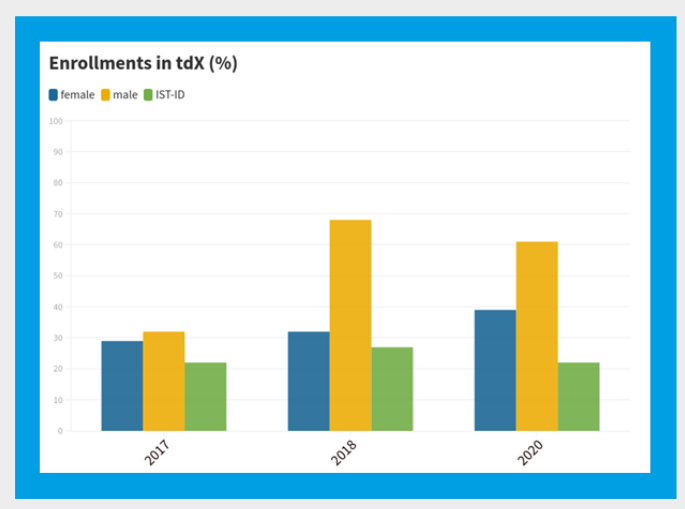
\includegraphics[width=.9\textwidth]{chaps/Images/enrollments_tdx.png}
    \caption{Taxas de inscrição nas várias edições do tdX.}
    \label{fig:enrollment_tdx}
\end{figure}

Na Figura 6, podemos ver a distribuição em cada ano da taxa de female, inscrição no tdX por género (female, male male) e a percentagem de inscritos com filiação IST (IST-ID), que neste caso é bastante inferior à percentagem
dos restantes inscritos, e bastante inferior aos valores das percentagens de inscrições com filiação IST no curso online droneX (ver Fig. 1 para os anos 2019 e 2020).

\begin{figure}
    \centering
    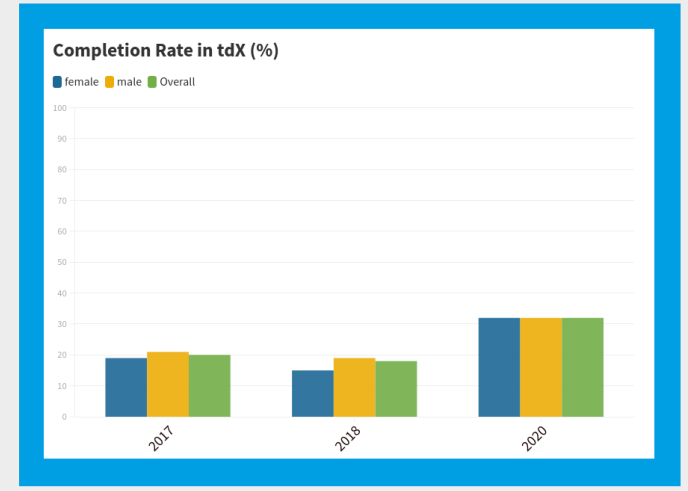
\includegraphics[width=.9\textwidth]{chaps/Images/completion_rate_tdx.png}
    \caption{Taxas de sucesso nas várias edições do tdX.}
    \label{fig:rate_tdx}
\end{figure}

Na Figura 7, podemos ver as taxas de sucesso (Completion rates) em cada Completion rates edição anual do tdX,as percentagens female, male género (female, female, por female, male male) e a overall percentagem Overall A partir dos dados total (Overall). referidos acima e da visualização das duas últimas figuras, podemos concluir que a maioria dos inscritos
no tdX são participantes externos ao IST de género masculino. As taxas de sucesso no tdX situam-se entre os 18\% e os 32\%, sendo que na última edição de 2020, todas as taxas de Overall female, male sucesso (Overall,
male) são iguais a este valor máximo de 32\%.

\begin{figure}
    \centering
    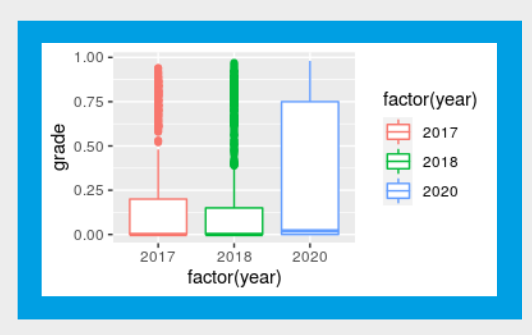
\includegraphics[width=.9\textwidth]{chaps/Images/boxplot_grade_tdx.png}
    \caption{Boxplot para a variável grade por fator year. Para cada caixa temos uma base que representa o primeiro quartil, um traço dentro da caixa que representa a mediana e o segundo quartil simultaneamente, e o topo da caixa que
representa o terceiro quartil. Os pontos isolados correspondentes às caixas vermelha e verde são outliers.}
    \label{fig:boxplot_grade_tdx}
\end{figure}

No diagrama boxplot da Figura 8, onde se pode ter uma leitura mais fina das taxas de sucesso relativas às notas obtidas pelos participantes, pode ver-se a existência de
muitos outliers outliers, principalmente nas duas primeiras edições 2017 e 2018 do tdX. Torna-se mesmo difícil de ler a mediana para esses dois anos, assim como a mediana
de 2020 que também está próxima de 2\% (numa escala de 0\% a 100\%) conferindo uma acentuada assimetria positiva nessas duas caixas. As caudas de distribuição, ou seja, as distâncias entre o terceiro quartil e o último
outlier, das notas para 2017 e 2018 também são grandes.

É importante recordar que a taxa de sucesso (Completion embora as referidas medianas se situem em valores muito baixos. Pode acontecer que o Peer Review resulte mais penalizante do que o tipo de avaliação usado no droneX. Na caixa respeitante à edição 2020 já não se visualizam outliers, outliers embora a dispersão das notas seja grande e o terceiro quartil fique nos 75\%. Recordamos que a última edição decorreu durante um período marcado pela pandemia Covid-19, em que o interesse e relevância de conteúdos online, em particular os MOOC, aumentaram substancialmente entre o público em geral. Os números de retenção desta edição 2020 do tdX
testemunham esta tendência.

\begin{figure}
    \centering
    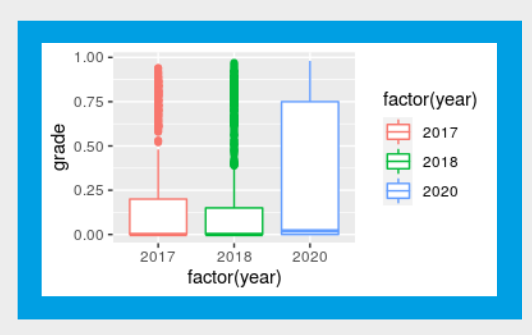
\includegraphics[width=.9\textwidth]{chaps/Images/boxplot_grade_tdx.png}
    \caption{Boxplot para as variáveis grade e gender poryear fator year.}
    \label{fig:boxplot_gender_tdx}
\end{figure}

No diagrama boxplot da Figura 9, verifica-se uma assimetria positiva muito acentuada dos dados de grade e gender (f=feminino e m= masculino) em relação ao fator year (anos 2017, 2018 e 2020) do curso online de tdX, principalmente nas caixas correspondentes às notas de participantes femininas. É possível ver com base na distribuição por género
das notas (numa escala de 0\% a 100\%) dos
participantes femininos e masculinos inscritos no tdX ao longo desses três anos, que as medianas se situam muito próximo dos 0\% em ambos os casos, sendo que na edição 2020 a mediana das notas dos participantes masculinos é próxima de 3\%.

A edição de 2020 foi aquela em que houve mais participantes inscritos que terminaram com sucesso as atividades de avaliação, em que o terceiro quartil das notas para o género masculino é de cerca de 75\%, igual ao valor do terceiro quartil global desta edição (ver Fig. 8).

\subsection{Conclusão sobre a experiência global do MOOC tdX}

Finalmente, concluímos que a maioria dos inscritos nas várias edições do tdX são participantes externos ao IST de género masculino.

Relativamente à prestação feminina nas várias edições do tdX , notamos que existe uma percentagem ligeiramente mais baixa de participantes femininas com sucesso no
MOOC (ver Fig. 7), excepto em 2020, em que a taxa de sucesso é igual para ambos os géneros. Eventualmente para esta tipologia de MOOC extracurricular faz mais sentido fazer outro tipo de análise com base noutros indicadores.

De modo geral, o público alargado, não obrigatoriamente académico, inscrito nas várias edições do curso online demonstrou estar satisfeito com as atividades de avaliação Peer Review), Review bem como com os conhecimentos adquiridos durante o curso.

Fica aqui a recomendação para se estudarem estratégias de captação e retenção de um público externo à escola, aplicando metodologias ativas que ajudem a aumentar as
taxas de sucesso nesta tipologia de MOOC transversal, com a ressalva que estas estratégias dependem muito do tópico
escolhido para o curso online, obviamente.

\subsection{Conclusão final das análises dos dados}

Terminada a análise separada sobre os dois MOOC com características distintas: o
curso “Simulação e Controlo de Drones”, droneX, dirigido principalmente a um
público de perfil “estudante IST”, e o curso “Transformação Digital”, tdX, dirigido a
um público alargado, conclui-se que a adesão às atividades de avaliação, enquanto
indicador do comportamento de adesão dos participantes a cada um dos tipos de
MOOC é também bastante distinta. Enquanto o droneX, aconselhado aos estudantes inscritos numa UC do Técnico Lisboa e usado para apoiar uma estratégia de flipped-classroom
flipped-classroom, consegue ter uma taxa média de sucesso na ordem dos 41\%, o curso “Transformação Digital”, dirigido a um público menos académico, eventualmente profissionais e potenciais empreendedores, tem uma taxa
média de sucesso de 23\%.

De referir que enquanto o número de inscritos no tdX foi sempre superior a mil inscritos, com uma maioria de inscritos externos ao IST, no droneX só na primeira edição de 2018 o número de inscritos foi superior a mil
participantes. 

Gostaríamos de acrescentar que a divulgação das várias edições do tdX beneficiaram de alguns apoios externos, enquanto no caso do droneX a divulgação foi mais interna ao IST, exceto na edição de 2018.

O público de ambos os MOOCs é predominantemente masculino (ver Fig. 1 e 6), com uma forte assimetria no caso do
droneX. Os inscritos no droneX, sendo alguns deles estudantes inscritos na UC “Controlo de Voo” (ver Fig. 5), são maioritariamente do género masculino. No entanto, as taxas de sucesso relativas (Fig. 2) e as notas obtidas (Fig. 4) pelas participantes femininas nas edições do droneX são em média superiores quando comparadas com as dos seus colegas masculinos. No caso do tdX, embora não sendo uma tendência muito acentuada, o comportamento global é o inverso (ver Fig. 7 e 9).

De modo geral, os participantes inquiridos no final de cada edição demonstraram estar satisfeitos com as atividades de avaliação e os conhecimentos adquiridos em ambos os casos, droneX e tdX (secções 2.3 e 3.3). Recordamos ainda que as últimas edições de ambos os cursos que ocorreram respetivamente, em abril e maio de 2020, durante um
Completion Rates período marcado pela pandemia Covid-19, não só tiveram taxas de sucesso (Completion Rates) mais elevadas (Fig. 2 e
7), como em geral as notas obtidas pelos participantes que terminaram com sucesso foram mais altas (Fig. 3 e 8). A apetência por este tipo de conteúdos validados, com boa qualidade gráfica, possibilitando uma formação gratuita e de fácil acesso deverá ainda aumentar nos próximos tempos.

Finalmente, gostaríamos de comentar com base nos resultados da nossa análise que um curso MOOC Técnico desenhado para um público com perfil “estudante IST de uma dada UC”, como o droneX, consegue captar e servir ainda uma comunidade mais alargada, como estudantes de outras UC, estudantes internacionais e/ou alumni que procuram aprofundar, rever ou alargar os seus conhecimentos sobre o tópico. Enquanto isso, um curso transversal,
como o tdX, para além do público externo ao IST, não obrigatoriamente académico, consegue também oferecer gratuitamente à comunidade da escola conteúdos extracurriculares de qualidade.

\section{O Projeto IgualdadeStem}

\subsection{Dados analisados}

\subsection{Evento Jornada das Mulheres}

\subsection{Artigos publicados}

\subsection{Trabalhos apresentados}







  Segundo a norma de formata{\c c}\~ao de teses e disserta{\c c}\~oes do
  Instituto Alberto Luiz Coimbra de P\'os-gradua{\c c}\~ao e Pesquisa de
  Engenharia (COPPE), toda abreviatura deve ser definida antes de
  utilizada.\abbrev{COPPE}{Instituto Alberto Luiz Coimbra de P\'os-gradua{\c
  c}\~ao e Pesquisa de Engenharia}

  Do mesmo modo, \'e imprescind\'ivel definir os s\'imbolos, tal como o
  conjunto dos n\'umeros reais $\mathbb{R}$ e o conjunto vazio $\emptyset$.
  \symbl{$\mathbb{R}$}{Conjunto dos n\'umeros reais}
  \symbl{$\emptyset$}{Conjunto vazio}

  \begin{longquote}
  Um exemplo de citação longa nas regras da ABNT (4cm de recuo e fonte menor)
  feita com o ambiente  \verb=longquote= The primary objective of this
  investigation was to determine the feasibility of detecting corrosion in
  aluminum Naval aircraft components with neutron radiographic interrogation
  and the use of standard corrosion penetrameters. Secondary objectives
  included the determination of the effect of object thickness on image quality,
  the defining of minimum levels of detectability and a preliminary investigation
  of a means whereby the degree of corrosion could be quantified with neutron
  radiographic data. 
  \end{longquote}

  \chapter{Revis\~ao Bibliogr\'afica}

  Para ilustrar a completa ades\~ao ao estilo de cita{\c c}\~oes e listagem de
  refer\^encias bibliogr\'aficas, a Tabela~\ref{tab:citation} apresenta cita{\c
  c}\~oes de alguns dos trabalhos contidos na norma fornecida pela CPGP da
  COPPE, utilizando o estilo num\'erico.

  \begin{table}[h]
  \caption{Exemplos de cita{\c c}\~oes utilizando o comando padr\~ao
    \texttt{\textbackslash cite} do \LaTeX\ e
    o comando \texttt{\textbackslash citet},
    fornecido pelo pacote \texttt{natbib}.}
  \label{tab:citation}
  \centering
  {\footnotesize
  \begin{tabular}{|c|c|c|}
    \hline
    Tipo da Publica{\c c}\~ao & \verb|\cite| & \verb|\citet|\\
    \hline
    Livro &  & \\
    Artigo &  & \\
    Relat\'orio &  & \\
    Relat\'orio &  & \\
    Anais de Congresso &  &
     \\
    S\'eries & & \\
    Em Livro & & \\
    Disserta{\c c}\~ao de mestrado &  &
      \\
    Tese de doutorado &  & \\
    \hline
  \end{tabular}}
  \end{table}
  
 \chapter{Investigações preliminares em motivação em ensino STEM}

\chapter{Trabalhos Relacionados}

  \chapter{M\'etodo Proposto}
  \chapter{Resultados e Discuss\~oes}
  \chapter{Conclus\~oes}

  \backmatter
  \bibliographystyle{coppe-unsrt}
  \bibliography{tese}

  \appendix
  \chapter{Algumas Demonstra{\c c}\~oes}
\end{document}
%% 
%%
%% End of file `example.tex'.
